\documentclass[a5paper]{book}% Tipo libro
% medidas del papel
\usepackage[paperwidth=15cm, paperheight=20cm]{geometry}
\usepackage[utf8]{inputenc}
\usepackage[T1]{fontenc}
\usepackage[spanish, es-tabla]{babel}
\usepackage{amsmath}
\usepackage{amssymb}
\usepackage{graphicx}
\usepackage{acronym}
\usepackage{float} 
\usepackage{mathpazo}
\usepackage{fancyhdr}
\usepackage{tikz,tkz-tab} %
\usepackage{easyReview} % revisar documentacion
\usepackage{tgbonum}
\usepackage{csquotes}
\usepackage{imakeidx}
\makeindex[columns=3, title=Alphabetical Index, intoc]
\usepackage[backend=biber, style=verbose, hyperref=true]{biblatex}
\usepackage{longtable}
\usepackage[table,dvipsnames]{xcolor}
\usepackage{titling}
\usepackage{needspace}

\addbibresource{bibliografia.bib}

\definecolor{enlace}{rgb}{0.6, 0.3, 0.6} % Un verde oscuro

\usepackage{hyperref}
\hypersetup{
    colorlinks=true,
    linkcolor=enlace,
    filecolor=magenta,      
    urlcolor=red,
    citecolor=blue,
    pdftitle={analisis regulatorio}}

\usepackage{tcolorbox, empheq} %
\tcbuselibrary{skins,breakable,listings,theorems}
% \usepackage[none]{hyphenat}% elimina la separacion de palabras

\usepackage{titlesec}   % customizing section titles
\usepackage{wasysym} % conjunto de simbolos

% formato del titulo
\titleformat{\chapter}[frame]
{\filright\bfseries}
{ \enspace  \fbox{CAPÍTULO \color{titlegreen}\thechapter} \enspace}
{1.1em}{\Large\bfseries\filcenter\color{titleblue}}

\usepackage{titlesec}
\usepackage{xcolor} % Para definir colores, opcional pero recomendado

% --- Definir un color para los títulos (opcional) ---
\definecolor{titleblue}{rgb}{0.0, 0.2, 0.4} % Un azul oscuro
\definecolor{titlegreen}{rgb}{0.0, 0.4, 0.4} % Un verde oscuro

% --- Formato de la SECCIÓN ---
% [block] -> El título ocupa su propio párrafo
% \Large\bfseries -> Letra grande y en negrita
% \thesection -> El número de la sección
% \titlerule[0.8pt] -> Una línea horizontal debajo del título
\titleformat{\section}[block]
  {\Large\bfseries\color{titleblue}}
  {\thesection.}
  {1em}
  {}

% --- Formato de la SUBSECCIÓN ---
% [hang] -> Formato estándar, el título puede ocupar varias líneas
% \large\bfseries -> Ligeramente más pequeño que la sección, en negrita
\titleformat{\subsection}
  {\large\bfseries\color{titlegreen}}
  {\thesubsection.}
  {1em}
  {}
  
% --- Formato de la SUB-SUBSECCIÓN ---
% \normalsize\itshape -> Tamaño normal, pero en cursiva para diferenciarlo
\titleformat{\subsubsection}[frame]
  {\normalsize\bfseries\color{titlegreen}}
  {\thesubsubsection.}
  {1em}
  {}

% --- Ajuste del espaciado ANTES y DESPUÉS de los títulos ---
% \titlespacing*{comando}{espacio-izq}{espacio-antes}{espacio-después}
% El asterisco (*) evita que se añada espaciado al inicio de una página.
\titlespacing*{\section}{0pt}{3.5ex plus 1ex minus .2ex}{2.3ex plus .2ex}
%\titlespacing*{\subsection}{0pt}{3.25ex plus 1ex minus .2ex}{1.5ex plus .2ex}
%\titlespacing*{\subsubsection}{0pt}{3.25ex plus 1ex minus .2ex}{1.5ex plus .2ex}
\titlespacing{\subsection}{12pc}{1.5ex plus .1ex minus .2ex}{1pc}
\titlespacing{\subsubsection}{12pc}{1.5ex plus .1ex minus .2ex}{1pc}

% estilo de cajas
\tcbset{width=0.6\linewidth,colback=gray!5!white,colframe=gray!75!black}


\fancyhf{} % Limpia todos los campos de encabezado y pie de página


% estilo de pagina
\pagestyle{fancy}

% Redefine \chaptermark para que no convierta a mayúsculas
% \markboth{texto para páginas izquierdas}{texto para páginas derechas}
% El segundo argumento vacío es para que no afecte a \rightmark (secciones)
\renewcommand{\chaptermark}[1]{\markboth{\thechapter. #1}{}}

% Asigna el contenido al encabe
\fancyhead[LO]{\small \leftmark}
\fancyhead[RE]{\small Capitulo \thesection}
\fancyhead[LE,RO]{\small página \bfseries\thepage   }
\fancyfoot[R]{\textit{\hyperref[sec:tabladecontendos]{tabla de contenido}}}            % clear page footer


\title{ANÁLISIS REGULATORIO}
\author{Alejandro Palacios}
% quita la indentacion de la primera línea  del parrafo.
\setlength{\parindent}{0cm}
% estilo de pagina
%\pagestyle{headings}

\renewcommand{\figurename}{\small\it  figura.}
% personalización de los caption
\usepackage[font=small,labelfont=bf,
labelsep=endash]{caption}

%% Para colocar un simbolo a los item
\renewcommand{\labelitemi}{\color{ForestGreen}{$\blacktriangleright$}}
%% para colocar color a las listas enumeradas
\renewcommand{\labelenumi}{\bfseries\color{red}{\theenumi .}} 

\begin{document}
	
\maketitle

  \begin{acronym}
  \acro{CND}{Centro Nacional de Despacho}
  \acro{COMTRADE}{Registros de falla originales}
  \acro{DNA}{Demanda no atendida}
  \acro{EDAC}{Esquema de Desconexión Automática de Carga}
  \acro{ENS}{Energía No Suministrada}
  \acro{FMECA}{Metodología de Análisis de Modos, Efectos de Falla y Criticidad (Failure Mode Effect and Criticality Analysis)}
  \acro{FNCER}{Fuentes no convencionales de energía renovable}
  \acro{LAC}{Liquidación y Administración de Cuentas}
  \acro{OR}{Operador de red}
  \acro{PENS}{Potencia Equivalente No Suministrada}
  \acro{RCM}{Mantenimiento Centrado en Confiabilidad}
  \acro{RETIE}{Reglamento técnico de las instalaciones eléctricas}
  \acro{SAEB}{Sistemas de Almacenamiento de Energía Eléctrica con Baterías}
  \acro{SDL}{Sistema de distribución local}
  \acro{SIN}{Sistema Interconectado Nacional}
  \acro{SP}{Sistema de potencia}
  \acro{STN}{Sistema de transmisión nacional}
  \acro{STR}{Sistema de transmisión regional}
  \acro{SOE}{Sequence Of Events}
  \acro{UPME}{Unidad de planeación minero energética}
\end{acronym}

\begin{center}
\begin{minipage}[c]{\linewidth}
            \textit{Este documento se desarrolla  un resumen regulatorio de las principales normas expedidas por los entes de control y  vigilancia en Colombia para el sector eléctrico, en  particular lo concerniente a la distribución de energía.}
\end{minipage}
\end{center}


\tableofcontents
\label{sec:tabladecontendos}
\clearpage

\printbibliography

\chapter*{ESTRUCTURA DE LA CONVOCATORIA}

\textit{Coordinar y controlar la operación y mantenimiento de la red de energía de acuerdo con las normas
 técnicas establecidas por la empresa, con el fin de garantizar su funcionamiento permanente.
}


 \section{Funciones del cargo}

 Las funciones del cargo Ingeniero de Operación y Mantenimiento  son las siguientes:
 
 \begin{itemize}
 \item  Analizar el funcionamiento del Sistema de Distribución local con el fin de programar y coordinar  las actividades relacionadas con la operación y/o Mantenimiento requeridas para garantizar la calidad del servicio y de la potencia.
\item  Coordinar y supervisar la ejecución de las diferentes actividades de operación y mantenimiento predictivo,  preventivo y correctivo de la red de servicios.
\item  Administrar adecuadamente los equipos, materiales Y herramientas requeridas para las actividades a realizar por el personal a su cargo.
\item  Propender por el cumplimiento de los indicadores de gestión establecidos para el área.
\item  Formular iniciativas tendientes a la optimización de los procesos y procedimientos de operación y mantenimiento de la red de servicios.
\item  Coordinar los diferentes grupos de trabajo para efectuar las actividades programadas en  el Sistema de Distribución Local de Energía.
\item  Elaborar informes de las actividades desarrolladas con la oportunidad y periodicidad requeridas.
\item  Realizar la supervisión, coordinación y control de las subestaciones, redes eléctricas y sus equipos asociados utilizando las herramientas y
medios de comunicación disponibles. 9. Participar en la supervision, coordinación, programación y configuración de los equipos de comunicación y/o operación de subestaciones.
\item  Coordinar oportunamente con el área de comercialización la prestación técnica del servicio de acuerdo con los respectivos contratos de compra
y venta de energía.
\item  Supervisar, revisar, verificar y controlar el uso de la infraestructura eléctrica por parte de los prestadores del servicio de Alumbrado Público y
operadoras de televisión por cable y telecomunicaciones, incluyendo la expansión y cobertura del servicio,
\item  Participar en la supervisión, coordinación y ajuste de las protecciones eléctricas instaladas en la conexión, la trensformación y el transporte del
Sistema de Distribución Local.
\item  Participar en la pianeacién, supervisión, coordinación, ejecución y control de las actividades propias de la medición de las fronteras comerciales de energía, tento a distancia como en el sitio.
\item  Presentar informes y estadísticas  periódicas de comportamiento del Sistema de Distribución Local con base en mediciones y parámetros establecidos en las normas y la reglamentación vigente.
\item  Mantener actualizado los manuales operativos del Sistema de Distribución Local.
\end{itemize}

\section{Conocimientos}

\subsection{CONOCIMIENTOS COMUNES}

\begin{itemize}
\item Derechos humanos
\item Gestión ambiental
\item Gestión de activos
\item Modelo integrado de pianeación y Gestión MIPG
\item Sistema de Gestión de calidad
\item Sistema de Gestion de salud y seguridad en el trabajo SG-SST
\item Ley anticorrupción
\item Élica empresarial
\item Ley de transparencia
\item Regulación y normetividad de servicios públicos
\item Ley disciplinaria de servidores públicos
\item Ley de acoso laboral
\item Reglamento intemo de trabajo
\item Modelo de operación por procesos
\item Portafolio de servicios
\item Gestión del riesgo
\end{itemize}

\subsection{CONOCIMIENTOS  BÁSICOS O ESENCIALES  POR NIVEL JERÁRQUICO}


\begin{itemize}
\item Gestión Contractual
\item  Gestión de Proyectos
\item Indicedores de Gestión
\item Formulación de Proyectos Bajo la Metodología General Ajustada (VIGA)
\end{itemize}

\subsection{CONOCIMIENTOS ESPECÍFICOS POR SUBPROCESO Y NIVEL JERÁRQUICO}

\begin{itemize}
\item «Reglamento Técnico de Instalaciones Eléctricas RETIE.
\item Compra de energía en el mercado de generadores.
\item «Infreestructura del sistema de distribución local de energia SDL.
\item Operación, funcionamiento y mantenimiento de las redes subterráneas y aéreas.
 su distribucion, protecciones, transformación y equipos.
\item «Regulación pertinente sobre la distribucién del servicio de energía.
\end{itemize}

  \section{COMPETENCIAS}

  \subsection{COMPETENCIAS COMPORTAMENTALES}

  \subsection{COMPETENCIAS FUNCIONALES}

  Las siguientes son las competencias funcionales :\\
  
  \begin{table}[H]
    \begin{tabular}{|p{0.5\linewidth}|p{0.5\linewidth}|}
      \hline
      \textbf{Actividad} &  \textbf{Competencia} \\\hline
      \textit{Distribuir energía} & Transportar energía eléctrica a través de las redes de distribución municipales o distitales, asegurando la distribucién conforme a parámetros del sistema eléctrico de energía    y la normativa asociada.\\\hline
      \textit{Evaluar y controlar la operación del sistema eléctrico de energía} &  Realizar el análiis y evaluación de la operación del sistema eléctico de energía, de acuerdo con parámetros de calidad, criterios técnicos y la normativa asociada. \\\hline
      \textit{Planificar la operación del sistema eléctrico de energía} & Planear la operación eléctrica de corto plazo de las redes del sistema eléctrico de energía y de los activos de  estas redes, conforme a los pianes definidos y en cumplimiento de la normativa asociada.\\\hline
    \end{tabular}
    \end{table}

  \section{RESPONSABILIDADES DEL ÁREA}

  Las siguientes son las responsabilidades del área:\\
  
  \begin{enumerate}
  \item Realizar la programación de las actividades sistemáticas del área funcional que permitan
 el cumplimiento de los objetivos y la implementación de las estrategias identificando su secuencia.
\item Analizar y aplicar la normatividad asociada a la operación del Sistema Eléctrico de Energía
 del Negocio de Energía.
\item Realizar el planeamiento de la operación de corto plazo del Sistema Eléctrico  de Energía, de acuerdo con lo definido en el marco regulatorio del sector eléctrico.
\item Realizar el inventario de la disponibilidad de los activos del Sisterna Eléctrico  de Energía y evaluar su estado para programar su  operación.
\item Coordinar con las dependencias adscritas a la Subgerencia de Distribución  la programación de los mantenimientos preventivos y correctivos del Sistema Eléctrico de Energía.
\item Coordinar con el Centro Nacional de Despacho el Estado  Operativo, la programación de mantenimientos preventivos y correctivos, la ejecución de racionamientos en el sistema interconectado del Sistema Eléctrico de Energía.
\item Coordinar, Analizar y evaluar las maniobras que sean presentadas en la Unidad.
\item Definir las necesidades de las compras de los elementos y equipos necesarios para ejecutar la operación del Sistema Eléctrico de Energía, estableciendo los parámetros  técnicos y términos de referencia.
\item Realizar  reportes de operación  de protecciones garantizar la operación  segura y confiable del sistema interconectado nacional.
\item Establecer los indicadores de gestión.
\item Calidad de potencia.
\item Garantizar por la regulación la descarga del sector de eléctrico información cotombiano.  desde los equipos de medición  utilizados para medir la calidad de la potencia en las variables solicitadas existencia.
\item Asegurar el almacenamiento de las interrupciones  y eventos  de sistema eléctrico.
\item Responder  por el almacenamiento de datos de la Calidad.
\item Proponer  soluciones medición.
\item Administrar  software, garantizando Gestionar su las funcionamiento tecnologías de de Operación manera confiable del Centro  y segura.
\item  Administrar y gestionar redes de comunicación.
\item Instalar  y mantener  la comunicación.
\item Adoptar los requerimientos de seguridad para la protección de activos del \ac{SDL},  que son consideradas críticas.
\item Realizar las labores de ingeniería necesarias para mantener operativas las aplicaciones  de tiempo real.
\item 
    \end{enumerate}
  
    \chapter{LISTA DE NORMAS Y REGLAMENTOS}

    \section{Leyes}

\begin{tabular}{|p{0.3\linewidth}|p{0.6\linewidth}|}
  \hline
  Legislación & DISPOSICIÓN \\\hline
  Ley 142 de 1994& Por la cual se establece el régimen de los servicios públicos domiciliarios y se dictan otras disposiciones.\\\hline
Ley 143 de 1994& Por la cual se establece el régimen para la generación, interconexión, transmisión, distribución y comercialización de electricidad en el territorio nacional– establece el régimen de las actividades del sector eléctrico colombiano\\\hline
  Resolución 1409 de 2012  & Trabajo seguro en alturas \\\hline
  Resolución 1348 de 2009 & Reglamento de salud ocupacional
en los procesos de generación, transmisión y distribución de
energía eléctrica en las empresas del sector eléctrico \\\hline
\end{tabular}

\section{Normatividad Calidad del servicio}

Las siguientes son referencias a la regulación con relación a la calidad del servicio  en el \ac{SIN}.\\\\

%% color de lineas
  \rowcolors{4}{gray!10!}{gray!40}
\begin{longtable}{|c|p{0.3\linewidth}|p{0.4\linewidth}|}

\caption{Reglamentos referentes a la calidad del servicio}
  % \label{tab:regcalidadservicio}
  \\\hline
   \rowcolor{black}\multicolumn{1}{|c|}{\color{white}\textbf{Resolución}}&\multicolumn{1}{|c|}{\color{white}\textbf{ALCANCE}} &  \multicolumn{1}{|c|}{\color{white}\textbf{DISPOSICIÓN}} \\\hline 
\endfirsthead

  \hline  \rowcolor{white}\multicolumn{3}{|l|}{\scriptsize \textit{\color{NavyBlue} \tablename\ \thetable{} -- continuación de la página anterior}} \\\hline
\hline \rowcolor{darkgray} \multicolumn{1}{|c|}{\color{white}\textbf{Resolución}} & \multicolumn{1}{c|}{\color{white}\textbf{ALCANCE}} & \multicolumn{1}{c|}{\color{white}\textbf{DISPOSICIÓN}}  \\\hline 
\endhead
\hline \rowcolor{white}\multicolumn{3}{|r|}{{\color{ForestGreen} \scriptsize \textit{\tablename\ \thetable{}\ ... Continua el la siguiente página}}} \\ \hline
\endfoot
\hline
\rowcolor{titleblue}\multicolumn{3}{|r|}{{ {\color{white}\scriptsize\textit fin de tabla}}} \\\hline
  \endlastfoot


  
  CREG 025 de 1995&  \ac{STN}, \ac{STR} y \ac{SDL} &  Por la cual se establece el \textbf{Código de Redes}, como parte del Reglamento de Operación del Sistema Interconectado Nacional.\\\hline

  CREG 070 de 1998 & \ac{SDL} & Establece reglas sobre la calidad del servicio en la distribución, introduciendo los conceptos de número y duración de las interrupciones. \\\hline

CREG 097 de 2008 &\ac{SDL} & Estableció una metodología integral para la remuneración de los Operadores de Red (OR) mediante establecimiento de los \textbf{cargos por uso} y un esquema de calidad del servicio más robusto. \\\hline
  
  CREG 011 de 2009 &  \ac{STN} y \ac{STR} & Estableció la metodología de remuneración de la actividad de transmisión de energía eléctrica, introduciendo un esquema explícito de calidad del servicio.\\\hline

  CREG 024 de 2013 &  \ac{STN} y \ac{STR}  & Modificó y complementó la metodología de remuneración del STN de la CREG 011 de 2009, ajustando aspectos relacionados con los planes de inversión y la valoración de los activos, manteniendo el enfoque de remuneración ligada a la disponibilidad.\\\hline

  CREG 015 de 2018& \ac{STR}  y \ac{SDL} &Por la cual se establece la metodología para la \textbf{remuneración} de la actividad de
distribución de energía eléctrica en el Sistema Interconectado
                                           Nacional.\\\hline

  CREG 36 de 2019 & \ac{STR}  y \ac{SDL}  & Es una modificación a la Resolución CREG 015 de 2018, específicamente en el artículo 1, y está relacionada con la regulación económica en el sector de energía y gas.\\\hline

   
\end{longtable}


\section{Normatividad Reporte de Eventos}

Los siguientes son la regulación con relación con relación al reporte de eventos.


%% color de lineas
  \rowcolors{4}{gray!10!}{gray!40}
\begin{longtable}{|c|p{0.3\linewidth}|p{0.4\linewidth}|}

\caption{Reglamentos referentes al reporte de eventos}
  % \label{tab:regcalidadservicio}
  \\\hline
   \rowcolor{black}\multicolumn{1}{|c|}{\color{white}\textbf{Resolución}}&\multicolumn{1}{|c|}{\color{white}\textbf{ALCANCE}} &  \multicolumn{1}{|c|}{\color{white}\textbf{DISPOSICIÓN}} \\\hline 
\endfirsthead

  \hline  \rowcolor{white}\multicolumn{3}{|l|}{\scriptsize \textit{\color{NavyBlue} \tablename\ \thetable{} -- continuación de la página anterior}} \\\hline
\hline \rowcolor{darkgray} \multicolumn{1}{|c|}{\color{white}\textbf{Resolución}} & \multicolumn{1}{c|}{\color{white}\textbf{ALCANCE}} & \multicolumn{1}{c|}{\color{white}\textbf{DISPOSICIÓN}}  \\\hline 
\endhead
\hline \rowcolor{white}\multicolumn{3}{|r|}{{\color{ForestGreen} \scriptsize \textit{\tablename\ \thetable{}\ ... Continua el la siguiente página}}} \\ \hline
\endfoot
\hline
\rowcolor{titleblue}\multicolumn{3}{|r|}{{ {\color{white}\scriptsize\textit fin de tabla}}}\\\hline
  \endlastfoot



  
  \end{longtable}
  

\begin{longtable}{|c|p{0.6\linewidth}|}
  \caption{Regulación CREG}\\
\hline \multicolumn{1}{|c|}{\textbf{Resolución}} & \multicolumn{1}{c|}{\textbf{DISPOSICIÓN}} \\ \hline 
\endfirsthead

\multicolumn{2}{c}
{\textit{ \tablename\ \thetable{} -- continuación de la página anterior}} \\
\hline \multicolumn{1}{|c|}{\textbf{Resolución}} & \multicolumn{1}{c|}{\textbf{DISPOSICIÓN}}  \\ \hline 
\endhead
\hline \multicolumn{2}{|r|}{{\textit{Continua el la siguiente página}}} \\ \hline
\endfoot
\hline
\multicolumn{2}{|r|}{{ {\scriptsize\textit  fin de tabla}}} \\
\hline
\endlastfoot


% \textbf{CREG 070 de 1998}& Codigo de Distribución \\\hline
% CREG 004 de 1999&Por la cual se aclaran y/o modifican las disposiciones establecidas en la Resolución CREG-051 de 1998, en la cual se aprobaron los principios generales y los procedimientos para definir el plan de expansión de referencia del Sistema de Transmisión Nacional y se estableció la metodología para determinar el \textbf{Ingreso Regulado} por concepto del Uso de este Sistema.\\\hline

CREG 039 de 1999& Por la cual se establecen las normas relacionadas
                  con las \textbf{pérdidas} de referencia en el
                  Sistema de Transmisión Nacional. \\\hline

CREG 080 de 1999& Por la cual se reglamentan las funciones de planeación, coordinación supervisión y control entre el \textbf{Centro Nacional de Despacho (CND)} y los agentes del SIN.\\\hline

CREG 022 de 2001&
Por la cual se modifican e incorporan las disposiciones establecidas
                  en la Resolución  CREG-051 de 1998, modificada por
                  las Resoluciones CREG-004 y CREG-045 de1999,mediante
                  las cuales se aprobaron los principios generales y
                  los procedimientos para definir el \textbf{plan de
                  expansión de referencia del Sistema de Transmisión
                  Nacional}, y se estableció la metodología para
                  determinar el \textbf{Ingreso Regulado} por concepto
                  del Uso de este Sistema.\\\hline
  
CREG 106 de 2006&Por la cual se modifican los procedimientos generales para la
                  asignación de\textbf{ puntos de conexión de
                  generadores} a los Sistema de Transmisión Nacional,
                  Sistemas de Transmisión Regional o Sistemas de
                  Distribución Local.\\\hline
  
% CREG 097 de 2008&  Por la cual se aprueban los principios generales y la metodología para el establecimiento de los \textbf{cargos por uso} de los Sistemas de Transmisión Regional y Distribución Local. \\\hline

% CREG 011 de 2009&Por la cual se establecen la metodología y \textbf{fórmulas tarifarías} para la remuneración de
% la actividad de transmisión de energía eléctrica en el Sistema de Transmisión
%                   Nacional.\\\hline
  
CREG 128 de 2010& Por la cual se establecen reglas para hacer la transición al nuevo esquema de
\textbf{calidad del servicio} en el Sistema de Transmisión Nacional adoptado por la
                  Resolución CREG-011 de 2009\\\hline

\textbf{CREG 156 de 2011}& Codigo de comercialización \\\hline
  
CREG 093 de 2012& Por la cual se establecen el reglamento para el \textbf{reporte de Eventos }y el procedimiento
para el cálculo de la \textbf{Energía No Suministrada}, y se precisan otras disposiciones relacionadas con la calidad del servicio en el Sistema de Transmisión Nacional\\\hline
  
CREG 094 de 2012& Por la cual se establecen el reglamento para el \textbf{reporte de Eventos} y el procedimiento para el cálculo de la \textbf{Energía No Suministrada}, y se precisan
                  otras disposiciones relacionadas con la calidad del servicio en los Sistemas de Transmisión Regional\\\hline
  
CREG 038 de 2014& \\\hline  
CREG 224 de 2016& Por la cual se establecen los criterios de
                  \textbf{confiabilidad} de la operación aplicables
                  para contingencias sencillas, como parte del Código
                  de Operación\\\hline

CREG 015 de 2018& Por la cual se establece la metodología para la \textbf{remuneración} de la actividad de
distribución de energía eléctrica en el Sistema Interconectado
                  Nacional.\\\hline
  
CREG 030  de 2018 & Por la cual se regulan las actividades de
                    autogeneración a pequeña escala y de generación
                    distribuida en el Sistema Interconectado
                    Nacional\\\hline
  
CREG 036 de 2019& Por la cual se modifican algunas disposiciones de la
                  Resolución CREG 015 de 2018.\\\hline
  
CREG 039 de 2019& Por la cual se establecen las normas relacionadas
                  con las \textbf{pérdidas} de referencia en el
                  Sistema de Transmisión Nacional.\\\hline
  
CREG 073 de 2019& Por la cual se modifica el artículo 2 de la Resolución CREG 224 de 2016 "por la cual
se establecen los criterios de \textbf{confiabilidad} de la operación aplicables para
                  contingencias sencillas, como parte del Código de Operación.\\\hline
  
CREG 28 del 2020 & Por la cual se aprueban las variables necesarias
                     para calcular los ingresos y cargos asociados con
                     la actividad de distribución de energía eléctrica
                     para el mercado de comercialización atendido por
                     Empresas Municipales de Cali
                     E.I.C.E. E.S.P.\\\hline
  
CREG 131 del 2020 & Medición AMI \\\hline
\end{longtable}




\begin{longtable}{|c|p{0.6\linewidth}|}
  \caption{Regulación CREG}\\
\hline \multicolumn{1}{|c|}{\textbf{ACUERDO}} & \multicolumn{1}{c|}{\textbf{DISPOSICIÓN}} \\ \hline 
\endfirsthead

\multicolumn{2}{c}%
{{\scriptsize\it\bfseries \tablename\ \thetable{} -- continuación de la página anterior}} \\
\hline \multicolumn{1}{|c|}{\textbf{ACUERDO}} & \multicolumn{1}{c|}{\textbf{DISPOSICIÓN}}  \\ \hline 
\endhead
\hline \multicolumn{2}{|r|}{{\scriptsize\it Continua el la siguiente página}} \\ \hline
\endfoot
\hline
\multicolumn{2}{|r|}{{\scriptsize\it fin de tabla}} \\
\hline
\endlastfoot

787 &
Por el cual se establecen las responsabilidades y los procedimientos a los cuales están
sujetos los agentes Transportadores, Operadores de Red, Generadores del SIN y el Centro
Nacional de Despacho –CND-, en la realización de informes referentes al \textbf{análisis de eventos}
que afecten la seguridad y confiabilidad del Sistema Interconectado Nacional –SIN\\\hline

963 & Mantenimientos de emergencia \\\hline

977 & Por el cual se aprueba el procedimiento para la \textbf{coordinación y ejecución} de las maniobras sobre activos de Uso del STN y STR y Conexión al STN \\\hline

1214 & Por el cual se aprueba el \textbf{Procedimiento para la entrada en operación comercial de proyectos de transmisión} que incluyan activos de uso del Sistema de Transmisión Nacional - STN -, del Sistema de Transmisión Regional - STR –, de usuarios conectados directamente al STN y de
recursos de generación \\\hline

1239 & Por el cual se aprueban las \textbf{Causas Detalladas para el Reporte de Maniobras Operativas}, Eventos y Cambios de Operatividad de activos del Sistema de Transmisión Nacional -STN- y del Sistema de Transmisión Regional -STR \\\hline

1254 & Por el cual se actualiza la definición y los \textbf{formatos de reporte de los parámetros técnicos de las plantas eólicas y solares fotovoltaicas} que se quieran conectar al Sistema de Transmisión Nacional STN, al Sistema de Transmisión Regional STR y al Sistema de Distribución Local
SDL \\\hline

1303 & Por el cual se actualizan los procedimientos para la \textbf{gestión integral de la demanda} \\\hline


\end{longtable}


\chapter{ESTRUCTURA DEL SECTOR ELÉCTRICO}

Los principios u objetivos de la prestación del servicio de electricidad son, de acuerdo al artículo 4 de  la ley  143 del 1994 \cite{LEY143}:

\begin{itemize}
\item\textit{ Eficiencia }: menor costo.
\item \textit{Calidad}: requisitos técnicos.
\item \textit{Continuidad}: deberá prestarse en caso de quiebra.
\item \textit{Adaptabilidad}: incorporación de nuevas tecnologías.
\item \textit{Neutralidad}: tratamiento igual para todos los usuarios.
\end{itemize}

El \ac{SIN} comprende la totalidad de las redes, subestaciones , generadores y usuarios se albergan en el \ac{SIN} , quien a su vez contiene el \ac{STN}, los  \ac{STR}'s y  los \ac{SDL}'s.

\section{STN: Sistema Transmisión Nacional}
Es el equivalente en el sector de transporte terrestre  a las autopistas nacionales, comprende las líneas, equipos de compensación, subestaciones, en el lado de baja y los correspondientes módulos de conexión de transformadores \cite{XM-2018-1}:
% \tcbox[colback=blue,colframe=red]{ejemplo}
\begin{center}
  \tcbox[colback=gray!40,colframe=gray!80]{V $\geq$ 220 kV.}
\end{center}

\begin{figure}[H]
  \centering
  \caption{Conformacion del STN}
  \includegraphics[width=0.5\linewidth]{STN_F}
\end{figure}

\section{STR: Sistema Transmisión Regional}
Esta conformado por los activos de conexión del \ac{OR} al \ac{STN}, conjunto de líneas, equipos y
subestaciones, con sus equipos asociados,  que no son usados en el \ac{SDL} y que operan en el nivel de tensión:
\cite{XM-2018-1}.

\begin{center}

  \begin{tcolorbox}[ title=STR:Nivel de tensión 4]
    {57.5 kV $\leq$ V < 220 kV }
\end{tcolorbox}
\end{center}

Existen dos \ac{STR}'s definidos por la reglamentación, estos son
:\\\\

\begin{itemize}
\item STR NORTE
\item STR CENTRO SUR
\end{itemize}

\begin{figure}[H]
  \caption{Partes del STR sur}
  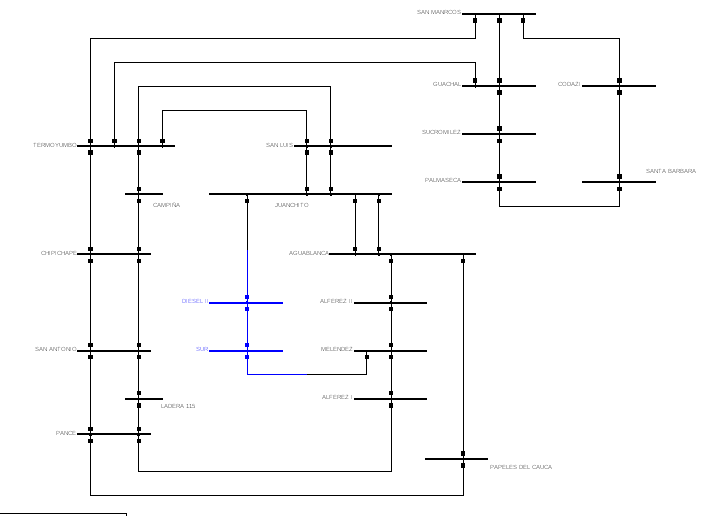
\includegraphics[width=\linewidth]{str}
\end{figure}
\section{SDL: Sistema Distribución Local}
Conjunto de líneas y subestaciones, con sus equipos asociados, que operan en los Niveles de Tensión 4, 3, 2 y 1 que no pertenecen las \ac{STR} y son usadas para el sistema de distribución local.

\begin{center}

  \begin{tcolorbox}[ title=SDL:Nivel de tensión 4]
    {57.5 kV $\leq$ V < 220 kV }
\end{tcolorbox}

  \begin{tcolorbox}[ title=SDL:Nivel de tensión 3]
    {30 kV $\leq$ V < 57.5 kV }
\end{tcolorbox}
\begin{tcolorbox}[ title=SDL:Nivel de tensión 2]
  { 1 kV $\leq$ V < 30 kV }
  \end{tcolorbox}
\begin{tcolorbox}[ title=SDL:Nivel de tensión 1]
  { V < 1 kV }
  \end{tcolorbox}
\end{center}

Por otra parte de acuerdo  al \ac{RETIE} \cite{RETIE2013} en el articulo 12, las instalaciones se pueden clasificar de acuerdo al nivel de tensión en función de su riesgo:\\\\
\begin{itemize}
\item Extra alta tensión > 230 kV
\item  230 kV  $\leqslant$ Alta tensión  > 57.5 kV .
\item 57.5 kV  $\leqslant$ Media tensión  > 1 kV .
\item Baja tensión < 1kV.
  \end{itemize}


\section{AREAS DE DISTRIBUCIÓN}
Conjunto de redes de Transmisión Regional y/o Distribución Local
destinado a la prestación del servicio en zonas urbanas y rurales, que
son operadas por uno o más Operadores de Red y que se conforman
teniendo en cuenta la cercanía geográfica de los mercados atendidos y
el principio de neutralidad establecido en la ley, y se establece que
debe existir un Cargo Único por Nivel de Tensión por cada ADD \cite{CREG1332013}.\\\\
\begin{itemize}
\item Oriente
\item  Occidente
\item  Sur 
                            \item  Centro
\end{itemize}

\section{AGENTES DEL SECTOR}
Los agentes del mercado son los encargados de producir, llevar y vender la energía al usuario final. Se clasifican en generadores, transmisores, distribuidores, comercializadores y administradores, según el rol que desempeñan.

\paragraph{Generadores}

Son los encargados de producir la energía por medio de centrales hidráulicas, térmicas y eólicas.
\paragraph{Transmisores}

Son los encargados de transportar largas distancias la energía desde las centrales eléctricas hasta las subestaciones de transformación a través de redes que operan a tensiones iguales o superiores a 220 kV.
\paragraph{Distribuidores}

Son los encargados de llevar la energía hasta el consumidor final a través de redes que operan a tensiones inferiores a 220 kV.
\paragraph{Comercializadores}

Son los encargados de la compra de energía eléctrica en el mercado mayorista y su venta a usuarios finales.

  
\chapter{PLANEACIÓN DE LA EXPANSIÓN DEL STN, STR Y SDL }

%La entidad encargada de realizar la planeación del \textbf{STN} es la \ac{UPME}.\\\\
La planeación de la operación se basa en tres ejes de acuerdo a la ley 143 \cite{LEY143} en el articulo 33, que son \textbf{confiable}, \textbf{segura} y con \textbf{calidad del servicio}.\\

\chapter{OPERACIÓN DEL SIN}

La operación del \ac{SIN}, comprende las siguientes componentes y esta a cargo del \ac{CND}:

\begin{enumerate}
\item Planeamiento Operativo
\item Despacho Económico
\item la coordinación
\item La supervición y control
\end{enumerate}

\section{PLANEAMIENTO OPERATIVO}

Se hace de forma integrada, garantizando seguridad, confiabilidad y
calidad de servicio \cite{CREG0251995}. Se descompone funcionalmente
como muestra la figura \ref{fig:planeamineto-operativo}\\\\

\begin{figure}[H]
  \centering
  \caption{Descomposición funcional y temporal del Planeamiento
    Operativo}
  \label{fig:planeamineto-operativo}
  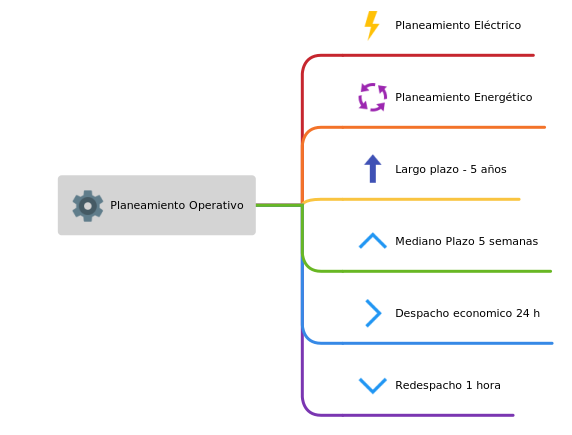
\includegraphics[width=1\linewidth]{planeamineto-operativo}
\end{figure}

\subsection{PLANEAMIENTO ENERGÉTICO}

Consiste en la planeación de la operación de los recurso energéticos,
hidráulicas y térmicos para la producción de energía eléctrica
\cite{CREG0251995}.

\section{DESPACHO ECONÓMICO}
Proceso mediante el cual se obtiene para un período de 24 horas, el programa horario de generación de los recursos del SIN despachados centralmente. Este despacho se efectúa con el criterio de minimizar el costo de atender la demanda.

En el numeral 1.3 del Código de Operación que hace parte del Código de Redes, adoptado mediante la Resolución CREG 025 de 1995, se definen las plantas despachadas centralmente de la siguiente forma:

\paragraph{Plantas Centralmente Despachadas}:

 Son todas las plantas de generación con capacidad efectiva mayor que 20 MW y todas aquellas menores o iguales a 20 MW que quieran participar en el Despacho Económico. 


\chapter{CONTROL DE TENSIÓN}

En estado estacionario las tensiones en las barras de 115 kV,
  110 kV y 220 kV, 230 kV no deben ser inferiores al 90\% ni
  superiores al 110\% del valor nominal. Para la red de 500 kV el
  voltaje mínimo permitido es del 90\% y el máximo es del 105\% del
  valor nominal \cite{CREG0251995}.\\\\

Para realizar el aumento de tensión se siguen con los pasos desarrollados en la figura:

\begin{figure}[H]
  \centering
  \caption{Aumento de tensión}
  \label{fig:aumentotension}
  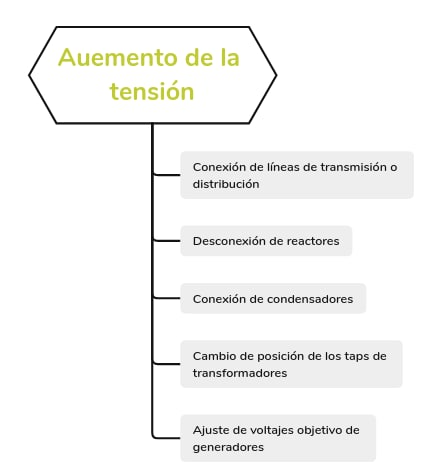
\includegraphics[width=0.8\linewidth]{aumentartension}
\end{figure}

Para reducir la tensión se procederá con los siguientes procesos:

\begin{figure}[H]
  \centering
  \caption{Reducción de  tensión}
  \label{fig:reducciontension}
  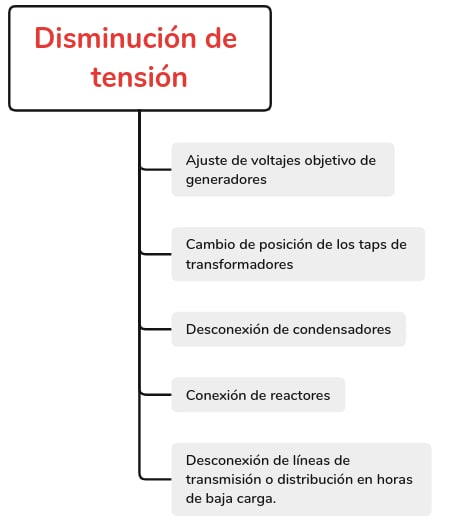
\includegraphics[width=0.8\linewidth]{reducirtension}
\end{figure}

  


\chapter{CONTROL DE FRECUENCIA}

De acuerdo al la resolución CREG 061 de 1996 se establece el esquema de desconexión automática de carga debe cumplir los siguientes criterios \cite{CREG0611996}:\\\\

\begin{itemize}
\item El disparo de la unidad de mayor capacidad del sistema no deberá activar la primera etapa de
desconexión
\item En ningún momento la frecuencia podrá ser inferior a 57.5 Hz
\item En contingencias se debe minimizar el tiempo que la frecuencia permanezca por debajo de 58.5 Hz
\item Después de 10 segundos de ocurrido un evento, la frecuencia del sistema deberá estar por encima
del umbral de la primera etapa del EDAC
\item Se deberá optimizar la cantidad de carga a desconectar en eventos, evitando al máximo la sobre
frecuencia, es decir, frecuencias superiores a 60 Hz después de ocurrido un evento
\end{itemize}

Para el año 2017 se aprobó el Esquema de Deslastre de Automático de
Carga EDAC por baja frecuencia que cubra un 40\% el total de la
demanda, distribuido en 8 etapas con desconexiones de carga del 5\%
\textbf{(Acuerdo 964} del 4 de mayo de 2017 ), El cual es ilustrado en
las figuras \ref{fig:edac}, \ref{fig:edac1} y \ref{fig:edac2}.

\begin{figure}[H]
  \centering
  \caption{Esquema EDAC}
  \label{fig:edac}
  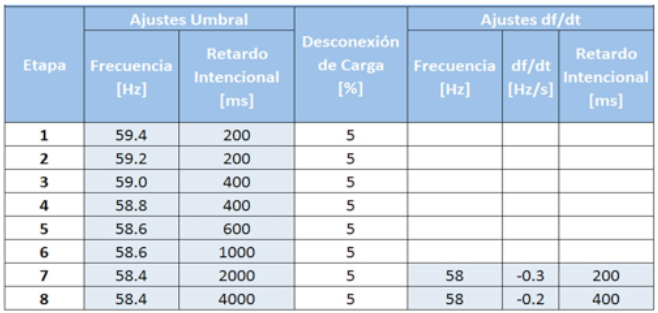
\includegraphics[width=0.8\linewidth]{esquema_edac}
\end{figure}

\begin{figure}[H]
  \centering
  \caption{Representación gráfica del esquema EDAC}
  \label{fig:edac1}
  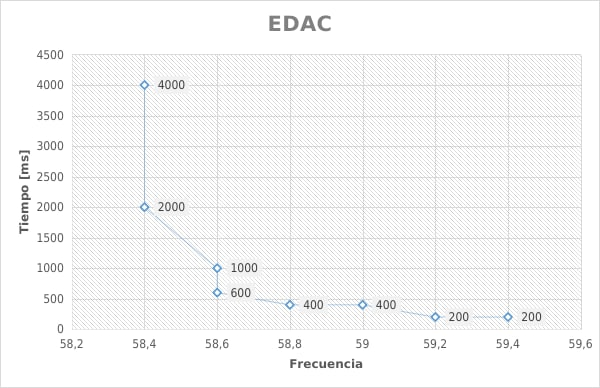
\includegraphics[width=0.8\linewidth]{EDAC1}
\end{figure}

\begin{figure}[H]
  \centering
  \caption{Representación gráfica del esquema EDAC}
  \label{fig:edac2}
  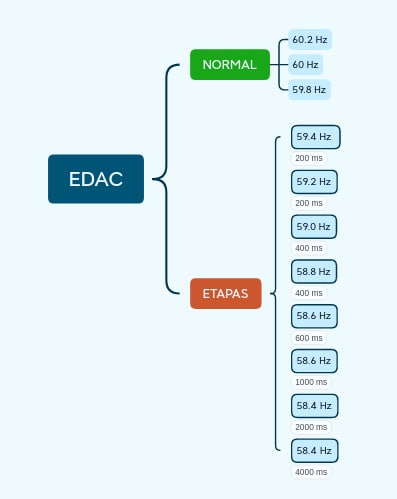
\includegraphics[width=0.8\linewidth]{EDAC}
\end{figure}


\

\chapter{PRONOSTICO DE LA DEMANDA}

Es un valor \textit{estimado} de la energía demandada en un mercado de
comercialización y su desagregación por centro de consumo. Este
pronóstico se propone por el CND antes del día míercoles y se corrige
por el OR hasta el viernes para si constituir el pronóstico oficial
del OR para su mercado de comercialización de la semana siguente ( de
lunes a Domingo). Durante la semana se pueden realizar ajustes antes
de las 7:30 a.m.\\\\
Para la estimación de la demand real el CND utiliza la siguiente
ecuación en un mercado de comencialización :\\\\
\[D_{real} = importacion + generacion - exportacion \]




\chapter{ESTABILIDAD}
 En el análisis de estado estacionario se consideran solo
  contingencias sencillas en las líneas de transmisión y en los bancos
  de transformadores 230/115 kV o 220/110 kV.\\\\
	
	
 Las corrientes e impedancias vistas por los relés vecinos, deben
  ser tales que no ocasionen la salida de elementos adicionales, lo
  cual originaría una serie de eventos en cascada.  En las barras
  principales del sistema de transmisión la tensión transitoria no
  debe estar por debajo de 0.8(p.u.) durante más de 500 mseg.\\\\
	
 Al evaluar la estabilidad del sistema de transmisión ante
  pequeñas perturbaciones, se debe chequear que los valores propios
  tengan componente de amortiguación. Si no hay amortiguación se deben
  ajustar apropiadamente los sistemas de control de las unidades de
  los equipos del SIN y como último recurso, limitar las
  transferencias por el sistema de transmisión.\\\\


                          \chapter{EVENTOS}

\section{REPORTE DE EVENTOS Y ENERGÍA NO SUMINISTRADA}

Cuando ocurre un evento programado (manenimiento ) o no programado (falla) se causa una
indisponibilidad total o parcial  sobre un activo \cite{CREG0942012}. Cuando esta
insisponibilidad causa un apagón en parte de la red se debe reportar la
 \ac{ENS} \cite{CREG0152018}, cuyo diagrama se muestra en la figura \ref{fig:ens}.

\begin{figure}[H]
  \centering
  \caption{Metodología del calculo del pronostico de la energía no
    suministrada}
  \label{fig:ens}
  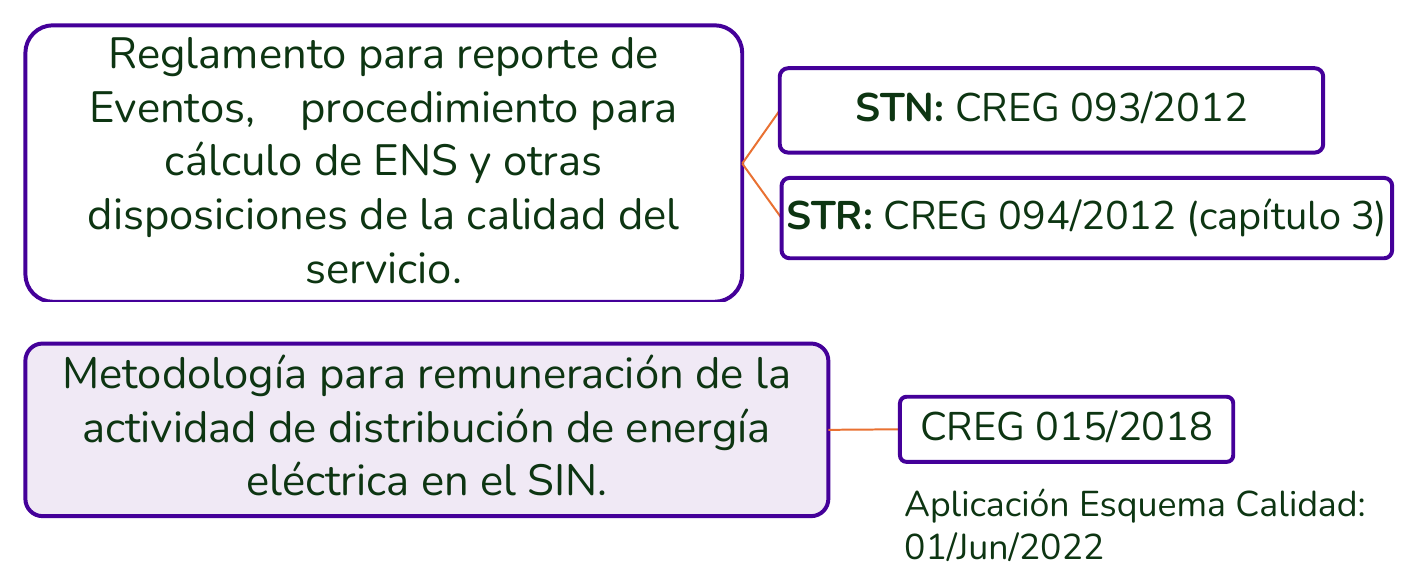
\includegraphics[width=\linewidth]{calculo_ens.png}
\end{figure}


La energía con la que se calcula la \ac{ENS} es la reportada por los
distintos comercializadores del mercado de comercialización.

  \section{ANÁLISIS DE EVENTOS}

El Acuerdo CNO 1617 actualiza el procedimiento para la elaboración de informes de análisis de eventos en el \ac{SIN}. El objetivo principal es identificar la causa raíz de los eventos no programados y determinar medidas para reducir o evitar su ocurrencia.\\\\

\begin{center}
\begin{tcolorbox}
La Ley 143 de 1994, en sus Artículos 34 y 38, establece las responsabilidades del Centro Nacional de Despacho (CND) en la coordinación, supervisión, control y análisis de la operación de los recursos del SIN, así como la obligación de las empresas generadoras, distribuidoras y operadoras de redes de suministro de información oportuna y fiel al CND y los CRD's.
\end{tcolorbox}
\end{center}

La \textbf{Resolución CREG 080 de 1999} define las responsabilidades del CND y los agentes del SIN en la realización de estudios sobre fallas y emergencias. La \textbf{Resolución CREG 083 de 1999} detalla la información obligatoria que los agentes deben adquirir y suministrar al CND, incluyendo registros cronológicos de eventos con alta resolución temporal y libre acceso a esta información. Las Resoluciones CREG 093 y 094 de 2012 requieren informes detallados para eventos no programados que superen un cierto umbral de PENS.\\\\

El Acuerdo 1617 introduce actualizaciones basadas en las Resoluciones \textbf{CREG 015 de 2018}, \textbf{036 de 2019} y \textbf{101023 de 2022}, incluyendo la responsabilidad de reporte de información por parte de los Operadores de Red (OR), los plazos para reportar el valor de la Energía No Suministrada (ENS) al LAC, y la inclusión de eventos no programados en los Sistemas de Almacenamiento de Energía Eléctrica con Baterías (SAEB). Los Anexos 1 y 2 detallan el procedimiento y los formatos específicos para la elaboración de estos informes.

\begin{figure}[H]
  \centering
  
  \caption{insumos para el análisis de eventos}
  \label{fig:insumoseventos}
  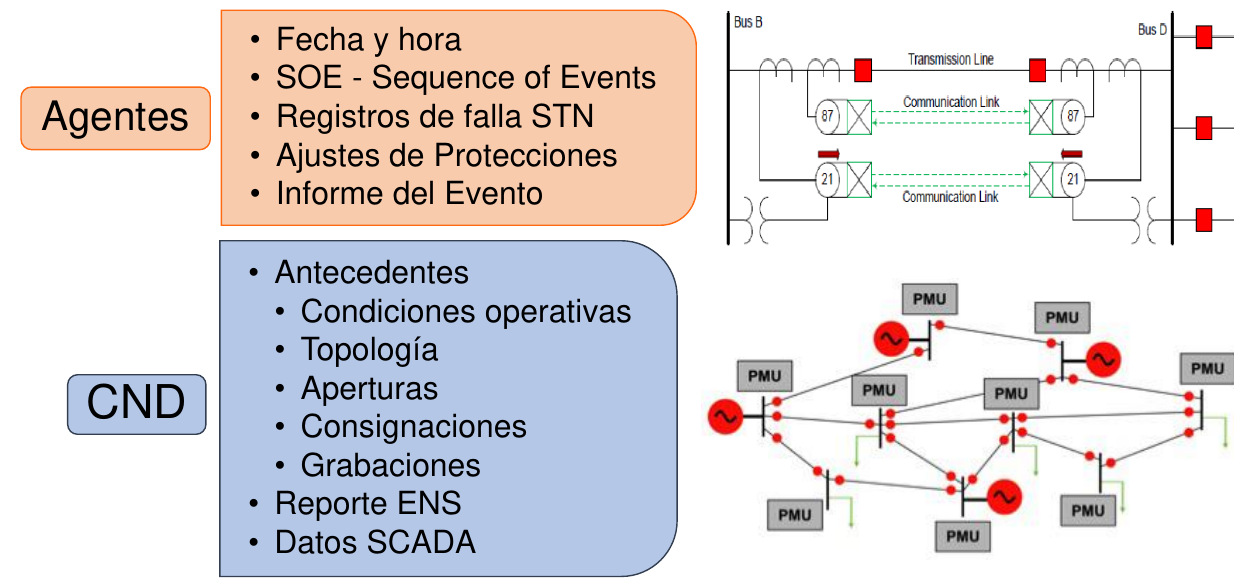
\includegraphics[width=0.8\linewidth]{insumos_eventos}
\end{figure}

\subsubsection{Responsables de los análisis y elaboración de informes}

\begin{itemize}
  
\item CND: Eventos en Activos de Uso del STN, Activos de Conexión al STN, Interconexiones Internacionales de nivel IV o superior, y otros que ameriten análisis.
    
  \item Transportadores de energía eléctrica en el \ac{STN} y/o Servicio de Conexión al \ac{STN}: Eventos en sus activos del \ac{STN}, incluyendo Interconexiones Internacionales con tensión igual o superior a 220 kV y Activos de Conexión al \ac{STN}.
  
  \item Operadores de Red (OR's): Eventos en los activos bajo su supervisión.
    
  \item Generadores: Deben suministrar información de plantas de generación si el \ac{CND} la requiere para sus análisis.

\end{itemize}



\subsection{Eventos a los que aplica el procedimiento de análisis}

\begin{itemize}
\item\textit{ Eventos no programados} que requieran análisis según Resoluciones CREG 093/2012, 094/2012 (Capítulo 3) y 015/2018.
\item Eventos en conexión internacional que originen \textit{separación de ambos sistemas eléctricos}.
    
\item Eventos que ocasionen la desconexión de \textit{2 o más} activos del STN (STN > N - 1).
    
\item Eventos en nivel de tensión IV o superior que generen la \textit{desconexión de todos los elementos} asociados a una barra o sección de barra.
    
\item Eventos que apliquen para análisis por \ac{SAEB}, cuando se cumplan los requerimientos regulatorios (\textbf{Resolución CREG 101023 de 2022}).
    
\item Eventos en el SIN que el CND considere que requieren análisis.
    
\item Eventos para los cuales los agentes soliciten análisis, previo acuerdo con el CND.

\end{itemize}
    
\subsection{Información a reportar por parte de los agentes}

 Identificación del activo, fecha y hora del evento, \ac{SOE} en formato editable, registros de falla originales (COMTRADE), ajustes de protecciones involucradas (si no están actualizados en la base de datos del CND), y cualquier información adicional pertinente.\\\\
Un informe detallado y completo del evento, siguiendo la estructura establecida en el Anexo 1.

\subsection{Estructura de los informes}

    Informe de Agentes: Resumen general, antecedentes (cuando aplique), análisis, causa (incluyendo activo causante y causas de desconexiones adicionales), operación de sistemas de protección, conclusiones (descripción del evento, operación de protecciones, DNA, ausencia de tensión, actuación EDAC/ESP/ESPS, otros hallazgos), acciones (ejecutadas y por ejecutar), recomendaciones, anexos.\\\\
    Informe del CND: Integra la información de los agentes, e incluye además: excursión de frecuencia en el resumen, recurrencia de inconvenientes en antecedentes, variación de frecuencia y cumplimiento de reglamentación en conclusiones, acciones y recomendaciones adicionales, referencias, y anexos opcionales (topología, secuencia del evento, condiciones operativas, otra información).\\\\
    Informes de Casos Especiales (Anexo 2): Aplicable a eventos específicos (retraso en consignación, disparo de generador, omisión de cierre, apertura manual no programada, SAEB, evento N-1 con PENS > 2\%). Tienen una estructura simplificada y no requieren revisión de agentes a menos que el CND identifique modificaciones necesarias.

\subsection{Plazos definidos para cada etapa del proceso (días hábiles a partir del día cero)}

Los plazos para la presentación del informe pueden agilizarse o prolongarse de acuerdo al los acuerdos con los agentes.

\begin{figure}[H]
  \caption{Plazo acuerdo CNO 1617 de 2022}
  \label{fig:plazo1617}
  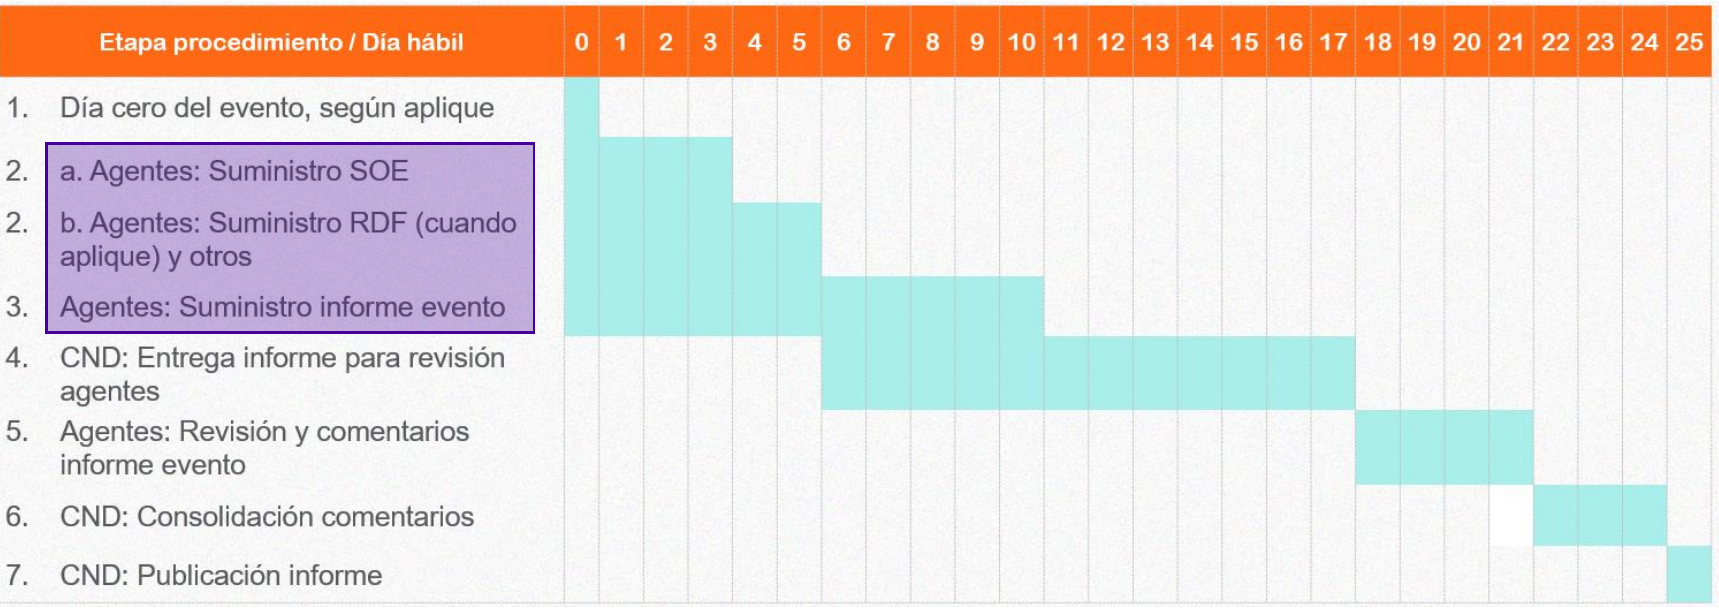
\includegraphics[width=\linewidth]{plazo16172022}
 \end{figure}

Suministro de SOE en el mínimo tiempo posible, RDF en 48-72 horas.\\\\
Reuniones para redefinir plazos, acuerdo con el CND para plazos adicionales de suministro de información con justificación escrita. El CND informará al CNO sobre estas prolongaciones.

\subsection{Seguimiento de Acciones}

    Responsabilidad de los agentes informar al CND la fecha de ejecución de acciones, número de consignación nacional y soportes técnicos.\\\\
    El CND mantendrá disponible el estado de las acciones, enviará trimestralmente un seguimiento al subcomité de protecciones y lo presentará en comités del CNO.\\\\
    Las acciones solo se podrán reprogramar con un plan de acción, fechas específicas y justificación.

\section{Preguntas de Quiz (10 preguntas de respuesta corta)}

\begin{enumerate}
\item ¿Cuál es la fecha de expedición y de entrada en vigencia del Acuerdo CNO 1617, y a qué acuerdo sustituye?
\item Según el Artículo 34 de la Ley 143 de 1994, ¿cuál es una función clave del CND?
\item ¿Qué tipo de información específica es obligatoria para los agentes del SIN según la Resolución CREG 083 de 1999 para el análisis de eventos?
\item ¿Qué umbral de PENS hace necesario un informe final detallado según las resoluciones CREG 093 y 094 de 2012, y quién es el responsable de publicarlo?
\item ¿Quiénes son los responsables de la recolección y el reporte de la información de eventos y de la calidad del servicio según la Resolución CREG 036 de 2019?
\item ¿Cuál es el objetivo principal del procedimiento establecido en el Anexo 1 del Acuerdo 1617?
    Mencione tres tipos de eventos a los que aplica el procedimiento de análisis de eventos del Acuerdo CNO 1617.
  \item Además de la identificación del activo y la fecha/hora, ¿qué otros dos tipos de información técnica mínima deben suministrar los agentes al CND para el análisis consolidado de eventos?
  \item ¿Cuál es la diferencia en el "día cero" para eventos relacionados con ENS/PENS y para otros eventos no programados según los plazos definidos?
  \item ¿Qué deben hacer los agentes si identifican que la información inicialmente reportada sobre el activo causante de un evento difiere del análisis detallado?
  \end{enumerate}
  
  \subsection{Clave de Respuestas del Quiz}

  \begin{itemize}

  \item El Acuerdo CNO 1617 fue expedido el 06 de Octubre de 2022 y entró en vigencia el 06 de Noviembre de 2022. Sustituye al Acuerdo 03/09/2015, Acuerdo 787.
  \item Según el literal b. del Artículo 34 de la Ley 143 de 1994, es función del CND "ejercer la coordinación, supervisión, control y análisis de la operación de los recursos de generación, interconexión y transmisión incluyendo las interconexiones internacionales".
  \item La Resolución CREG 083 de 1999 establece como obligatoria la remisión de: a) Registro sobre la secuencia cronológica de eventos (SOE) y b) Por cada evento, fecha y hora con resolución de un (1) ms, identificación del elemento que cambió de estado y el estado final del dispositivo.
  \item Un informe final detallado es necesario cuando el PENS supere el 2\%. El CND es el responsable de elaborar y publicar este informe sobre ENS.
  \item Los Operadores de Red (OR) son los responsables de la recolección y el reporte de la información de eventos y la requerida para la aplicación de las disposiciones de calidad del servicio. En todo caso, el responsable de la calidad y oportunidad de la información es el agente a quien se le remuneran los activos.
  \item El objetivo principal es establecer un procedimiento para la elaboración de los informes de análisis de eventos en el Sistema Interconectado Nacional (SIN) por parte del CND y los agentes del SIN.
  \item Tres tipos de eventos a los que aplica son: a) Eventos no programados que requieran análisis según Resoluciones CREG 093/2012, 094/2012 (Capítulo 3) y 015/2018; b) Eventos en conexión internacional que originen separación de ambos sistemas eléctricos; c) Eventos que ocasionen la desconexión de 2 o más activos del STN (STN > N - 1); d) Eventos en nivel de tensión IV o superior, que generen la desconexión de todos los elementos asociados a una barra o sección de barra; e) Eventos que apliquen para análisis por SAEB. (Cualquiera de estas tres son válidas).
  \item Los agentes deben suministrar el SOE (Sequence Of Events) en formato editable y los registros de falla originales (sin editar), en formato COMTRADE o estándar sustituto.
    Para eventos que deban ser analizados según ENS/PENS (numeral 'a'), el día cero (0) es la fecha en la cual el CND publica el cálculo de Energía No Suministrada (ENS). Para los demás criterios (numerales 'c', 'd', 'f', 'g'), el día cero es el día de ocurrencia del evento.
  \item Si el activo que dio origen al evento difiere de la información inicialmente reportada, los agentes son responsables de solicitar al CND las modificaciones de la información correspondiente en dicho reporte de eventos, en caso de que aplique.
    \end{itemize}

\subsection{Preguntas de Formato Ensayo}
\begin{itemize}
\item Compare y contraste las responsabilidades del CND y de los Agentes del SIN en la elaboración y suministro de información para los informes de análisis de eventos, detallando cómo se complementan sus roles según el Acuerdo 1617.
   
\item  Analice la importancia de los plazos establecidos en el Acuerdo 1617 para la eficiencia y la efectividad del proceso de análisis de eventos. Discuta las "Consideraciones para agilizar los plazos" y "Consideraciones para prolongar los plazos", y cómo estas buscan equilibrar la celeridad con la profundidad del análisis.
    
\item Describa la evolución de la regulación del sector eléctrico que ha llevado a la expedición del Acuerdo 1617, haciendo referencia a al menos cuatro resoluciones CREG mencionadas y explicando cómo cada una contribuye al marco regulatorio actual del análisis de eventos.
\item Explique en detalle la estructura requerida para un informe de análisis de eventos elaborado por los agentes del SIN, tal como se describe en el numeral 3.2 del Anexo 1. Incluya los componentes obligatorios y su propósito en la identificación de la causa raíz y las acciones correctivas.
\item Discuta el rol de los "Casos Especiales" en el procedimiento de análisis de eventos, tal como se definen en el numeral 3.4 y el Anexo 2. Explique por qué ciertos eventos se clasifican como especiales y cómo su tratamiento difiere del procedimiento estándar para eventos más complejos.
\end{itemize}
\subsection{Glosario de Términos Clave}

\texttt{\begin{itemize}
  \item Acuerdo CNO 1617: Documento que actualiza el procedimiento para la elaboración de informes de análisis de eventos en el Sistema Interconectado Nacional (SIN).
  \item Activo: Se refiere a cualquier elemento o componente del Sistema Interconectado Nacional, según las definiciones de las Resoluciones CREG 011 de 2009 y CREG 015 de 2018.
  \item Agente Generador: Empresa encargada de la producción de energía eléctrica dentro del SIN.
  \item Agentes del SIN: Las empresas generadoras de electricidad, las distribuidoras y las que operan redes de interconexión y transmisión dentro del Sistema Interconectado Nacional.
  \item CND (Centro Nacional de Despacho): Entidad central en el SIN responsable de la coordinación, supervisión, control y análisis de la operación del sistema, incluyendo la gestión de información de eventos.
  \item CNO (Consejo Nacional de Operación): Órgano que aprueba acuerdos y procedimientos relacionados con la operación del SIN.
  \item COMTRADE: Estándar para el intercambio de datos de registros de falla, utilizado para los registros oscilográficos en el análisis de eventos.
  \item Consignación Nacional: Proceso formal de autorización para retirar activos del SIN de operación por mantenimiento u otras razones programadas.
  \item CRD’s (Centros Regionales de Despacho): Entidades regionales que apoyan al CND en la coordinación y operación del SIN.
  \item CREG (Comisión de Regulación de Energía y Gas): Organismo regulador que emite resoluciones y normativas para el sector eléctrico en Colombia.
  \item Demanda No Atendida (DNA): Cantidad de energía que la demanda requirió pero no pudo ser suministrada debido a una interrupción o limitación del sistema.
  \item Día Cero (0): El punto de inicio para el conteo de plazos en el procedimiento de análisis de eventos, cuya definición varía según la clasificación del evento.
  \item Disturbio: Evento no planeado que produce una condición anormal en el SIN, como una perturbación o un cambio inesperado en el Error de Control de Área (ACE).
  \item EDAC (Esquema de Desconexión Automática de Carga): Mecanismo de control automático que desconecta bloques de carga para preservar la estabilidad del SIN ante perturbaciones significativas.
  \item ENS (Energía No Suministrada): Energía que no pudo ser entregada a los usuarios finales debido a interrupciones o fallas en el sistema, medida en unidades de energía (e.g., MWh).
  \item Evento: Condición anormal o perturbación en el SIN que requiere análisis, según las Resoluciones CREG 093 de 2012 y CREG 015 de 2018.
  \item ESP/ESPS (Esquemas de Protección / Esquemas de Protección Especiales): Conjuntos de protecciones diseñados para operar ante condiciones específicas del sistema, más allá de la protección básica de los equipos.
  \item Falla: Un evento en el SIN que implica un cortocircuito, una interrupción o una condición de operación anormal de un activo.
  \item Interconexiones Internacionales: Conexiones eléctricas que permiten el intercambio de energía entre el SIN de Colombia y sistemas eléctricos de países vecinos.
  \item Interruptor: Dispositivo de conmutación capaz de interrumpir y establecer corrientes en condiciones normales y anormales del circuito.
  \item LAC (Liquidación y Administración de Cuentas): Se refiere al proceso o entidad encargada de la compensación por energía no suministrada o por otros aspectos económicos del mercado eléctrico.
  \item Ley 143 de 1994: Ley Marco Eléctrica de Colombia que establece los principios generales y las regulaciones del sector energético.
  \item Operador de Red (OR): Empresas encargadas de la operación y el mantenimiento de las redes de transmisión regional (STR) y distribución local (SDL).
  \item PENS (Potencia Equivalente No Suministrada): Una medida de la potencia no entregada a los usuarios, utilizada para clasificar la severidad de los eventos y determinar la necesidad de informes detallados.
  \item Protecciones: Conjunto de dispositivos y sistemas diseñados para detectar fallas o condiciones anormales en el sistema eléctrico y operar equipos (como interruptores) para aislar la falla y proteger la integridad del sistema y los activos.
  \item Registros Oscilográficos: Grabaciones de alta velocidad de las magnitudes eléctricas (corrientes, tensiones) durante un evento, cruciales para el análisis de fallas.
  \item SAEB (Sistemas de Almacenamiento de Energía Eléctrica con Baterías): Tecnologías de almacenamiento de energía que utilizan baterías para gestionar el suministro y la demanda en el SIN.
  \item Seccionador: Dispositivo de conmutación utilizado para aislar eléctricamente una parte del circuito para mantenimiento o seguridad, no diseñado para interrumpir corrientes de falla.
  \item SEP (Sistema Eléctrico de Potencia): Conjunto de elementos interconectados (generación, transmisión, distribución y consumo) que conforman el sistema eléctrico.
  \item SIN (Sistema Interconectado Nacional): La red eléctrica principal de Colombia que conecta las diferentes regiones y fuentes de generación con los centros de consumo.
  \item SOE (Sequence Of Events): Un registro cronológico y detallado de la operación de equipos y protecciones durante un evento, crucial para reconstruir la secuencia de los hechos.
  \item SSPD (Superintendencia de Servicios Públicos Domiciliarios): Organismo que supervisa y controla la prestación de los servicios públicos, incluyendo la energía eléctrica.
  \item STN (Sistema de Transmisión Nacional): La parte de la red de transmisión de energía eléctrica que opera a las tensiones más altas (iguales o superiores a 220 kV), gestionada por los transportadores.
  \item STR (Sistema de Transmisión Regional): La parte de la red de transmisión de energía eléctrica que opera a tensiones intermedias (menores de 220 kV y no parte del SDL), gestionada por los Operadores de Red (OR).
  \item Subcomité de Protecciones: Un comité técnico dentro del CNO que se encarga de analizar y dar concepto favorable a las actualizaciones relacionadas con los sistemas de protección.
\end{itemize}}
  \section{DEMANDA NO ATENDIDA}

  Es un valor \textit{estimado} de la energía no entregada a la carga
  debido a eventos programados o no programados. Para ello se emplean
  los eventos diarios reportados en ENERGIS.\\\\

  \section{ENERGÍA NO SUMINISTRADA}

  La energía no suministrada es la dejada de entregar a partir de la
  ocurrencia de un evento en el \ac{STR} \cite{CREG0152018}. Esta se
  puede calcular de acuerdo a la siguiente expresión: \cite{CREG0942012}\\\\

  \[ ENSMH_{j,h} = PRN_{j,h} - DE_{j,h} \]

  \begin{tabular}{p{0.2\linewidth} p{0.7\linewidth}}
    Donde :\\\\& \\
    $ENSMH_{j,h}$& Es la energía no suministrada en  un mercado de comercialización a una hora dada \\
    $PRN_{j,h}$ & Es el pronóstico nuevo de la demanda\\
    $DE_{j,h}$ & Es la demanda de electricidad \\
  \end{tabular}\\

  
\hspace{1cm}
  Los datos para el calculo de estos valores son almacenados en la
  base de datos del CND por un tiempo máximo de cinco años en el
  aplicativo HEROPE. Es resposabilidad del OR reportar esta
  información\\\\
  
\chapter{CARGABILIDAD}
\section{CARGABILIDAD DE CIRCUITOS}
 La \textit{máxima transferencia por las líneas} se considera
  como el mínimo valor entre el límite térmico de los conductores,
  máxima capacidad de los transformadores de corriente, el límite de
  transmisión por regulación de voltaje y el límite por estabilidad
  transitoria y dinámica \cite{CREG0251995}.\\\\

  La operación del sistema dentro de los límites de carga
  determinados , exceptuando la sobrecarga de
  transformadores, se consideran como operación normal. Fuera de ellos
  el sistema se considera que está en estado de alerta o de
  emergencia.\\\\
  
Para los circuitos se tendrá como criterio de carga máxima, la
permitida por el conductor en caso de realimentaciones. En condiciones
óptimas  no se debe superar el 70 \% de la capacidad térmica del
conductor \cite{MANOPEMCALI}. En la figura \ref{fig:capacidad_conductores_emcali} se
muestra la capacidad de los conductores empleados en EMCALI.

\begin{figure}[H]
  \centering
  \caption{Capacidad de conductores EMCALI}
  \label{fig:capacidad_conductores_emcali}
  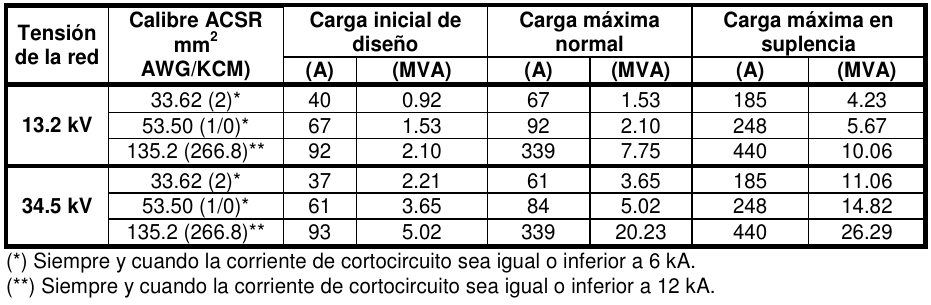
\includegraphics[width=\linewidth]{aereos_emcali}
\end{figure}

\begin{figure}[H]
  \centering
  
  \caption{capacidad de corriente de los conductores}
  \label{fig:ampacidad}
  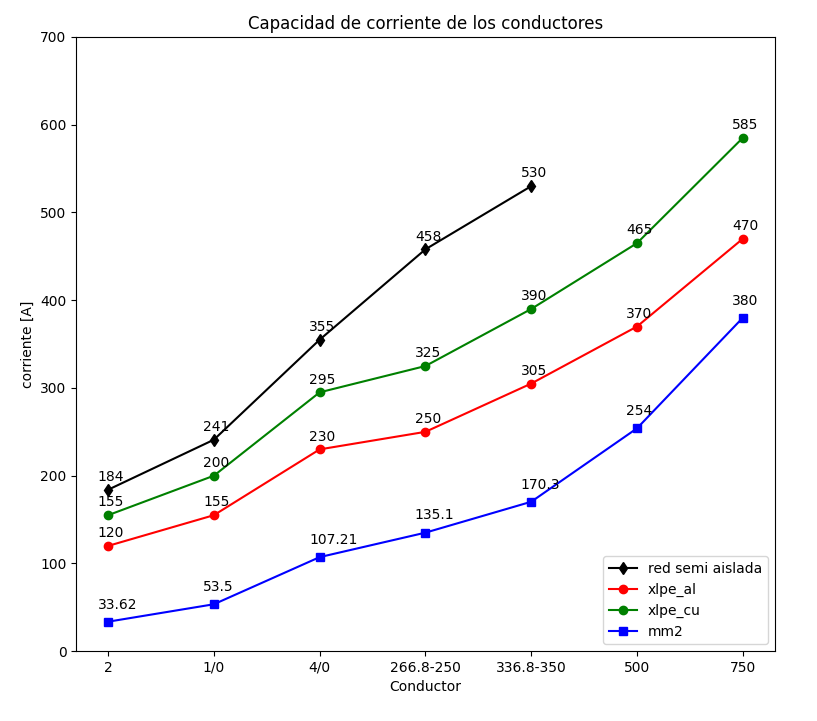
\includegraphics[width=\linewidth]{capacidad_corriete}
\end{figure}


\section{CARGABILIDAD DE LOS TRANSFORMADORES}

Para los transformadores de potencia, en ningún caso se debe superar
el 100\% de la capacidad nominal de cada uno. La capacidad real
operativa de cada transformador estará determinada por las condiciones
de funcionamiento de los sistemas de refrigeración \cite{MANOPEMCALI}.


\chapter{CONTINGENCIAS}

Una contingencia se refiere a una situación de emergencia donde se puede llegar a perder parte del sistema de potencia. El sistema de distribución debe estar en capacidad de seguir suministrando carga en caso de una de las siguientes contingencias \cite{EMCALI2007}:

\begin{enumerate}
	\item Pérdida de una subestación con dos o tres transformadores.
	\item Pérdida de una barra de 13.2 kV
	\item Pérdida de un transformador.
	\item Pérdida de un tramo de circuito.
	\item Pérdida de un interruptor de circuito.
	\item Pérdida del tramo subterráneo.
\end{enumerate}

\subsubsection{Pérdida de una Subestación con Dos o Tres Transformadores}

En caso de pérdida de una subestación estandard se pierden
aproximadamente 77 MVA de carga en 13.2 kV (con una cargabilidad del 91\%), las cuales deben ser atendidos por las subestaciones adyacentes mediante transferencias de carga  de carga en la red.\\\\
 En una subestación promedio, el valor esperado de carga en cada transformador de 41.75 MVA es de 38 MVA y en cada transformador de 28 MVA es de 26 MVA.\cite{EMCALI2007}.\\\\

En caso de realizar realimentaciones totales de una subestación , de acuerdo a la cargabilidad del momento se recomienda seguir el siguiente plan de contingencia:

\subsubsection{Pérdida de una Barra de 13.2 kV}

 transferir las secciones de los alimentadores a alimentadores de otras
subestaciones

\subsubsection{Pérdida de un Transformador}

\subsubsection{Pérdida de un Tramo de Circuito}

\subsubsection{Pérdida de un Interruptor de Circuito}

\subsubsection{Pérdida del Tramo Subterráneo}

\section{DESCONEXIONES PREVENTIVAS}

Cuando se presentan retardos en la entrada  en operación de líneas , transformadores u otros activos pertenecientes al \ac{STN} o \ac{STR},  de acuerdo al análisis eléctrico  realizado por el \ac{CND},  este ordenará la desconexión preventiva de la demanda de un \ac{OR} cuando se presentan los siguientes casos: \cite{CREG2242016} \\\\

\begin{itemize}
\item Se desconectará el 20\% de la carga cuando un evento no programado o contingencia sencilla  \footnote[1]{Cada uno de los eventos no programados que causan la no operatividad de una línea, un transformador o un banco de transformadores del STN o del STR.}  sobre un activo (linea , transformador u otro ) pueda 
  \end{itemize}

Cantidad de carga en MW que se desconectaría de las redes del SIN ante la ocurrencia de una contingencia resultante de la operación de los equipos de protección del sistema, actuación de esquemas suplementarios, apertura de elementos por superación de límites operativos de equipos declarados por los agentes o por las instrucciones operativas del CND derivadas de la ocurrencia de una contingencia. La desconexión correctiva de demanda es estimada por el CND, con base en la mejor información disponible para los análisis eléctricos.





\chapter{CALIDAD DEL SERVICIO}

La calidad del servicio  es una variable que representa las características técnicas del servicio que el usuario persive. Esta afectada por los eventos que ocurren en
el \ac{SIN}, los cuales pueden o no dejar demanda no atendida.

\begin{figure}[H]
  \centering
  \caption{Evento de gran magnitud}
  \label{fig:eventogranmagnitud}
  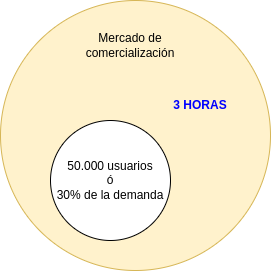
\includegraphics[width=0.6\linewidth]{evento_gran_magnitud}
\end{figure}

Es preciso indicar que las compensaciones por calidad se sustentan en fundamentos regulatorios
de acuerdo con el sistema o nivel de tensión, como se muestra en la

\begin{tabular}{llp{0.25\linewidth}p{0.25\linewidth}}
  \hline
Resolución CREG& Sistema & Nivel de tensión & Aplicación \\\hline
  097 de 2008 & STR & & Actual  \\\hline
  \end{tabular}

\section{CALIDAD DEL SERVICIO EN EL STR}





los reportes realizados por el \ac{OR} al \ac{CND} son los que se muestran en la figura:


\begin{figure}[H]
  \centering
  
  \caption{Reportes enviados al CND}
  \label{fig:reportes_transmision}
  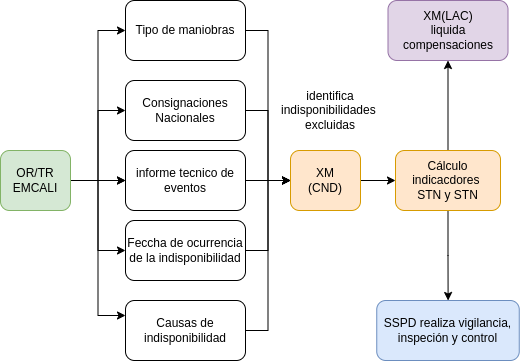
\includegraphics[width=\linewidth ]{reportes_transmision}
\end{figure}

El ingreso de cada agente se ve afectado por las siguientes variables:\\\\

\begin{itemize}
\item Cuando las in-disponibilidades superan las máximas horas anuales de in-disponibilidad ajustadas
\item Las in-disponibilidades debidas a catástrofes no superen los seis meses
\item La energía no suministrada no debe exceder los límites.
\item Un activo que supero las máximas horas de in-disponibilidad ajustada no se puede permitir que deje otros activos no operativos
\end{itemize}


Para realizar los procedimientos descritos (eventos programados y no programados ) se tendrán en cuenta los siguientes plazos, cada uno contado a partir de las 24:00 horas del día de operación:\\\\

\begin{tabular}[H]{|p{4cm}|c|c|}
  \hline
Actividad & Responsable&Plazo (h)\\\hline
Ingreso de reporte de eventos &Agente&12\\\hline
Validación y publicación de listado de inconsistencias&
CND&
36\\\hline
Solicitud de modificación de información&
Agente&
60\\\hline
Respuesta a solicitudes de modificación&
CND&
72\\\hline
  \end{tabular}

  Los siguientes grupos de activos utilizados en la prestación del servicio de distribución de energía eléctrica en el STR, no deberán superar, en una ventana móvil de doce meses, el número de máximas horas anuales de indisponibilidad, MHAI, que se definen para los grupos de activos identificados en la tabla \cite{CREG0152018}.\\\\

  \begin{tabular}[H]{|p{6cm}|c|}
    \hline
Grupos de Activos&
MHAI\\\hline
Conexión del OR al STN&
65\\\hline
Equipo de compensación&
18\\\hline
Línea del STR&
38\\\hline
Barraje sin bahías de maniobra&
15\\\hline
Barraje con bahías de maniobra&
30\\\hline

  \end{tabular}

  Los siguientes  grupos de activos incluyen las bahías de conexión :\\\\
  \begin{itemize}
  \item Conexión del OR al STN
  \item Equipo de compensación
  \item Línea del \ac{STR}
  \end{itemize}

  Las máximas horas anuales de indisponibilidad  se reducen en 0.5 h cuando se presenten unas de las siguientes situaciones:
  
  \begin{figure}[H]
    \centering
    \caption{incremento de las maximas horas anuales de indisponibilidad}
    \label{fig:mhaia}
    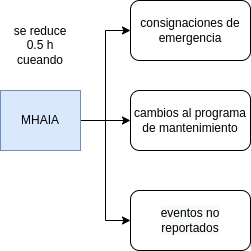
\includegraphics[width=0.6\linewidth]{MHAIA}
  \end{figure}
  
Las horas que un activo  se encuentra  in disponible durante un mes, se pueden calcular como \cite{CREG0152018}:

  \[ HID_{m,u} = \sum_{x=i}^{n}(H_{i,u}*(1-CAPD_{i,u}))  \]

    La \textbf{capacidad de los activos} tras suceder un evento queda establecido  como se muestra en la figura \ref{fig:capacidad} \cite{CREG0152018}:

    \begin{figure}[H]
      \centering
      \caption[capacidad]{Capacidad de los activos tras ocurrir un evento}
      \label{fig:capacidad}
      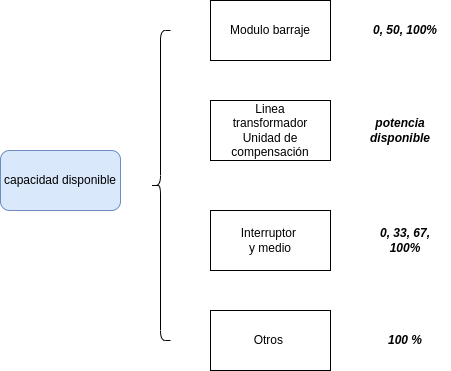
\includegraphics[width=\linewidth]{capacidad_eventos}
    \end{figure}

En caso de un mantenimiento mayor el cual requiere más horas de las programadas en las máximas horas anuales de indisponibilidad, se tienen en cuenta las horas que se muestran en la figura \ref{fig:mayor} \cite{CREG0152018}.

    \begin{figure}[H]
      \centering
      \caption{máximas horas anuales de indisponibilidad para los mantenimientos mayores}
      \label{fig:mayor}
      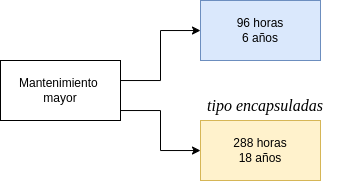
\includegraphics[width=\linewidth]{mantenimoento_mayor}
    \end{figure}
  


    \section{CALIDAD DEL SERVICIO EN EL SDL}

    \begin{figure}[H]
  \centering
  \caption{mapa conceptual del proceso de calidad del servicio}
  \label{fig:esquema}
  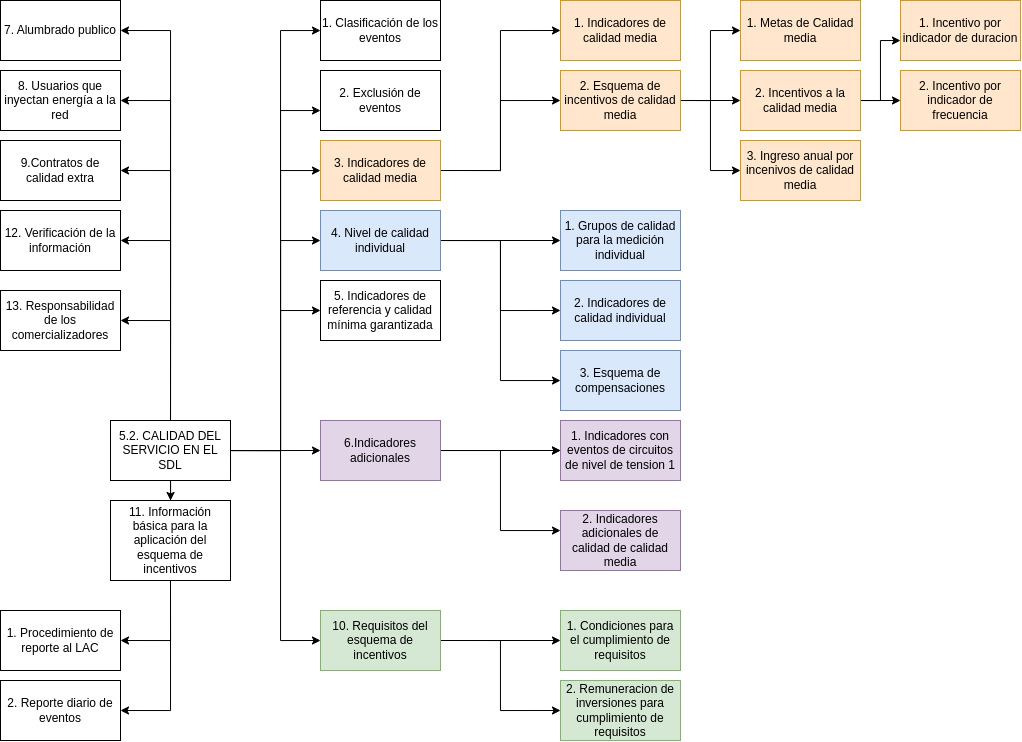
\includegraphics[width=\linewidth]{mapa_calidad_sdl}
\end{figure}

    El esquema de incentivos y compensaciones corresponde al nivel mínimo que deben cumplir las empresas dentro del plan regulatorio de metas para el mejoramiento de la calidad, el cual en concordancia con lo dispuesto por los artículos 58 y 59 de Ley 142 de 1994, estarán sujetos al seguimiento, vigilancia y control de la SSPD \cite{CREG0152018}.\\\\
    Para efectos de cumplir con la prestación continua de un servicio de buena calidad artículo 136 de la Ley 142 de 1994, o cualquier norma que la modifique o la adicione, los OR deberán abstenerse de incurrir en cualquiera de los siguientes escenarios \cite{CREG0152018}:

    \begin{figure}[H]
      \centering
      \caption{Eventos excluidos}
      \label{fig:excluidos}
      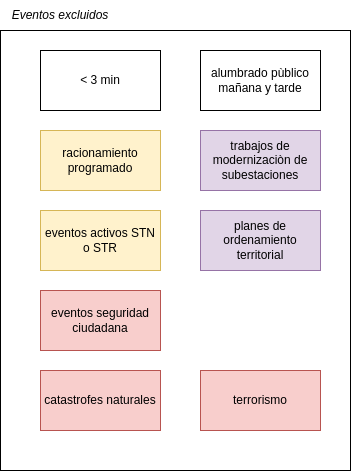
\includegraphics[width=\linewidth]{exclusiones_sdl}
    \end{figure}

    para su estudio los usuarios también se pueden agrupar en grupos
    de calidad lo cual depende de dos variables: los índices de
    ruralidad \textbf{IR} e índice de riesgo de falla \textbf{IRF},
    entonces se tienen seis posibles grupos de calidad como lo muestra
    la gráfica \ref{fig:gruposcalidad} \cite{CREG0152018}.\\\\

    \begin{figure}[H]
      \centering
      
      \caption{grupos de calidad}
      \label{fig:gruposcalidad}
      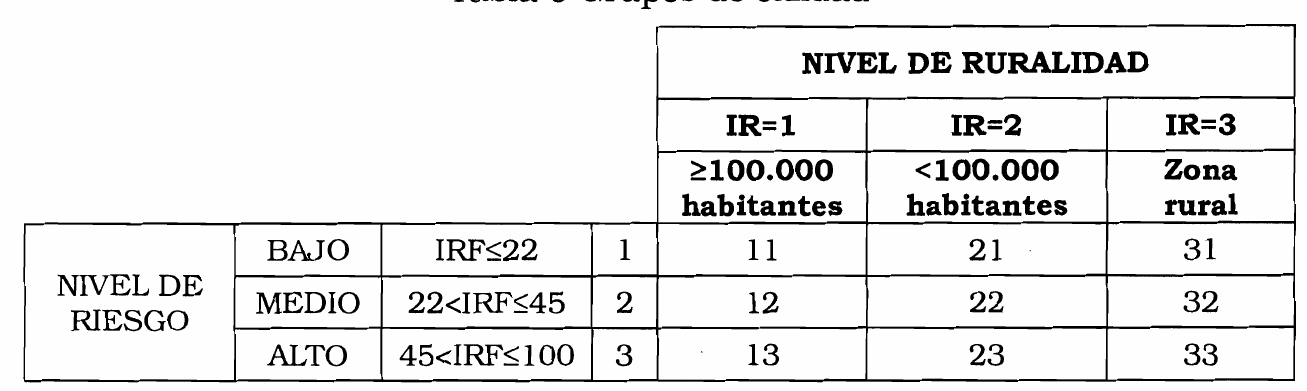
\includegraphics[width=\linewidth]{grupos_de_calidad}
    \end{figure}

    \section{INDICADORES DE CALIDAD DE DURACIÓN}

    La calidad  de energía  promedio o media del sistema en cuanto a duración puede ser establecida en función del indicador \textbf{SAIDI} (Indice de duración media de interrupción del sistema [\textit{System average interruption duration index}]) como se muestra a continuación:

    \[ SAIDI  = \sum_{m=1}^{12}\dfrac{\sum(D*NU)}{60*UT}   \left[  \dfrac{h}{usuario} \right]  \]\\
    Donde:\\\\
    \begin{tabular}[H]{p{1cm}p{8cm}}
      
      $D$ & {\small\it es la duración del evento en minutos}\\
      $NU$ & {\small\it es el número de usuarios afectados por el evento} \\
      $UT$ &  {\small\it  usuarios totales del \ac{SDL}} \\
    \end{tabular} \\\\

    Para determinar los valores a los que debe llegar se debe establecer las \textbf{metas anuales} para este indicador,  la cual se denomina \textbf{SAIDI\_M},  se parte de un valor  histórico de referencia denominado \textbf{SAIDI\_R}, para el caso de EMCALI  este valor es \textit{19.122 h} \cite{CREG0282020}.\\\\
    
    El indicador para medir la calidad individual anual para un usuario se conoce  como $DIU$, y el indicador mensual se conoce como $DIUM$ y se puede obtener a partir de:\\\\


    \[ DIU = \sum_{ma=m-11}^{m}DIUM  \]
    \[ DIUM = \sum_{i}^{IT}D\]
    En este caso la  duración del evento es en horas.\\\
    
    El valor  es límites que no se deberían sobrepasar se conocen como \textbf{DIUG}.\\\\

    Para los eventos momentáneos de debe calcular el \textbf{CAIDI}

    \begin{figure}[H]
      \centering
      \caption{Valores de SAIDI}
      \label{fig:valoressaidi}
      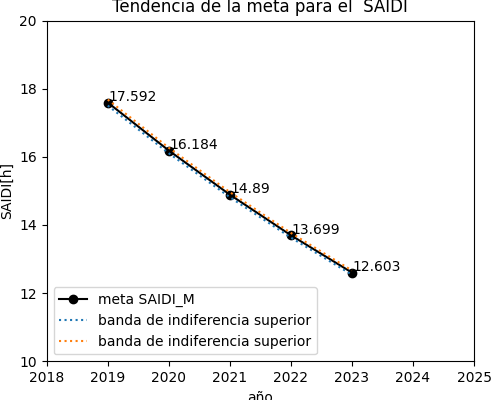
\includegraphics[width=\linewidth]{meta_saidi}
    \end{figure}
    
    \section{INDICADORES DE CALIDAD DE FRECUENCIA}
    
    \[ SAIFI  = \sum_{m=1}^{12}\dfrac{\sum(NU)}{UT}   \left[  \dfrac{veces}{usuario} \right]  \]

    Para elaborar los indicadores de calidad  individual de frecuencia se toma el de manera anual el $FIU$ y mensualmente el $FIUM$ como se muestra a continuación:\\\\

    \[  FIU = \sum_{ma=m-1}^{m} FIUM \]

    \[ FIUM = \sum_{i=1}^{IT} F\]

    El  valor límite que no se debería sobrepasar se conocen como  \textbf{FIUG}.

    Para los eventos momentáneos (nenores a 3 min) se debe reportar el \textbf{MAIFI} el cual se calcula como:
    \[ MAIFI = \dfrac{\sum_{i=1}^{n}NU }{UT}\]
    
    

    \chapter{PROTECCIONES ELÉCTRICAS}

    Las siguientes son las características generales de las protecciones eléctricas:\\\\
\begin{itemize}
	\item Alta Confiabilidad: Probabilidad de no omitir disparos
	\item Alta Seguridad: Probabilidad de no tener disparos indeseados
	\item Selectividad: Desconectar sólo lo fallado, evitando trasladar los efectos de las fallas a otros lugares del STN. 
	\item Rapidez: El tiempo de operación debe ser lo suficientemente corto de modo que garantice mantenerla estabilidad del sistema
        \end{itemize}

        En los sistemas eléctricos de los distribuidores, grandes consumidores y transportadores, el tiempo máximo de despeje de falla de la protección principal, desde el inicio de la falla hasta la extinción del arco en el interruptor de potencia, no debe
        ser mayor que 150 milisegundos.\\\\

        Los tipos de relés de sobre corriente se pueden clasificar como se muestra en la figura:

\begin{figure}[H]
      \centering
      
      \caption{tipos de relés en función al tipo de operación}
      \label{fig:tiporele}
      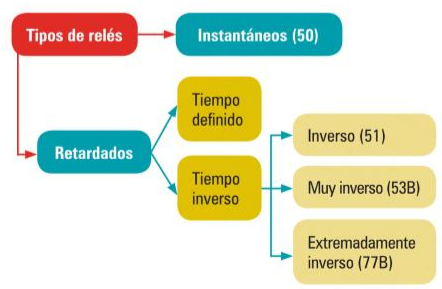
\includegraphics[width=\linewidth]{tipos_rele}
    \end{figure}



    \section{PROTECCIONES DEL TRANSFORMADOR}

    \begin{figure}[H]
      \centering  
      \caption{Protecciones del transformador de potencia}
      \label{fig:proteccionestrafo}
      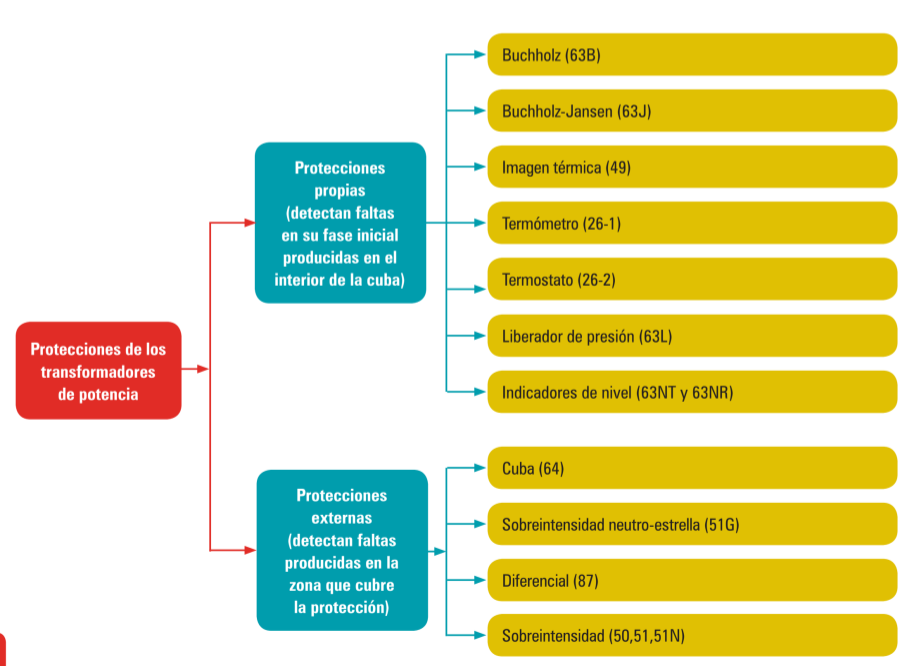
\includegraphics[width=\linewidth]{proteccion_trafo}
    \end{figure}

        \begin{figure}[H]
      \centering  
      \caption{diagrama protecciones del  transformador de potencia}
      \label{fig:diagramatrafo}
      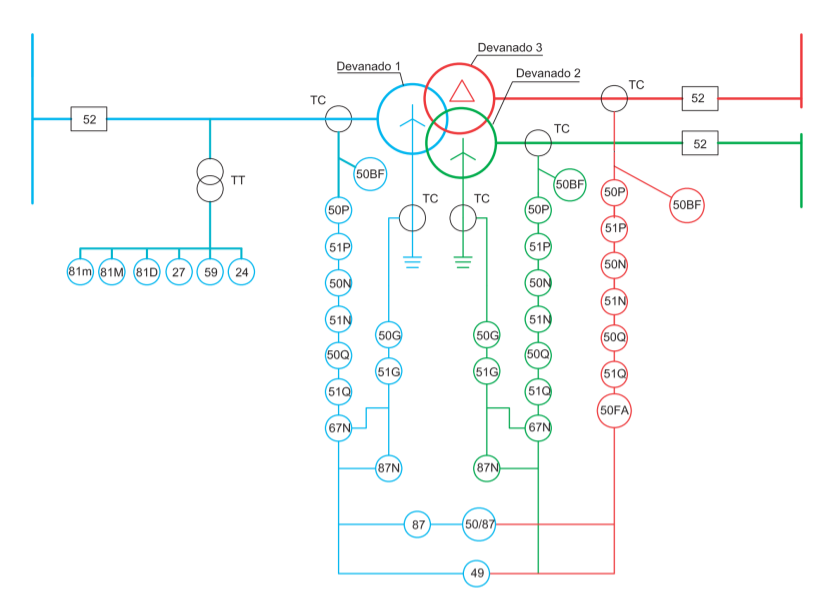
\includegraphics[width=\linewidth]{diagramapttrafo}
    \end{figure}

           \begin{figure}[H]
      \centering  
      \caption{diagrama protecciones del  transformador de potencia}
      \label{fig:diagramatrafo1}
      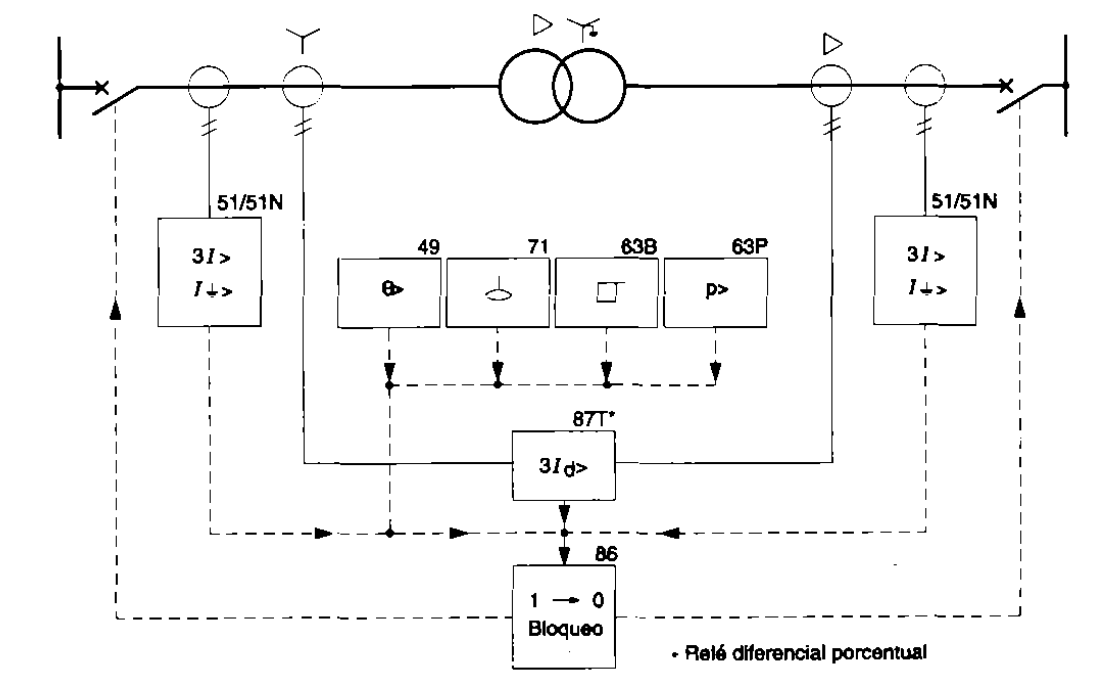
\includegraphics[width=\linewidth]{proteccion_trafo_1}
    \end{figure}

En la figura \ref{fig:zonas_diferencial},  se puestra el traslape de
zonas en la protección diferencial.
    
    \begin{figure}[H]
      \centering
      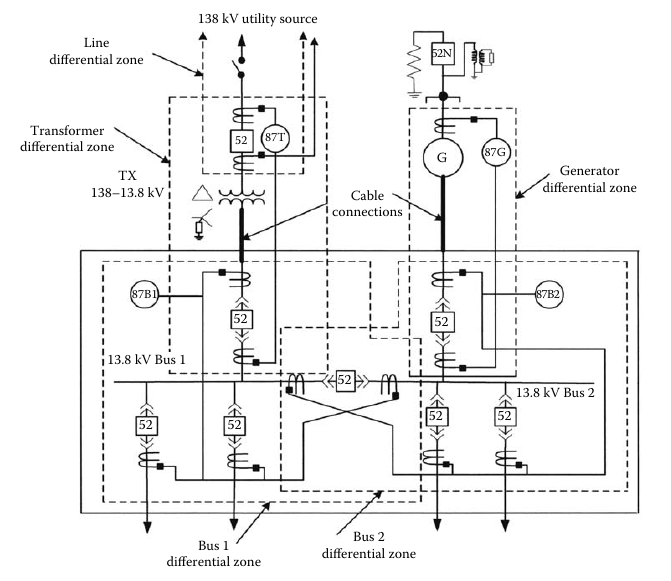
\includegraphics[width=\linewidth]{diferencial_tranformador}
      \caption{solapamiento de las zonas de protección diferencial}
      \label{fig:zonas_diferencial}
    \end{figure}
    



\begin{longtable}{|c|p{0.8\linewidth}|}
  \caption{Señales del transformador}\\
\hline \multicolumn{1}{|c|}{\textbf{Señal}} & \multicolumn{1}{c|}{\textbf{DESCRIPCIÓN}} \\ \hline 
\endfirsthead

\multicolumn{2}{c}%
{{\it \tablename\ \thetable{} -- continuación de la página anterior}} \\
\hline \multicolumn{1}{|c|}{\textbf{Señal}} & \multicolumn{1}{c|}{\textbf{DESCRIPCIÓN}}  \\ \hline 
\endhead
\hline \multicolumn{2}{|r|}{{\textit{Continua el la siguiente página}}} \\ \hline
\endfoot
\hline
\multicolumn{2}{|r|}{{ {\scriptsize\textit  fin de tabla}}} \\
\hline
\endlastfoot

  \small
  24 & Sobreexitación \\\hline
  23 & Temperatura \\\hline
  27 & Sub tensión \\\hline
  32 & Potencia direccional \\\hline
46 & secuencia negativa\\\hline
  49 & Térmico\\\hline
  50P & Sobre corriente instantánea de fase \\\hline
  50 & Sobre corriente \\\hline
  50BF & Fallo en breaker \\\hline
  50Q & Sobre corriente istantánea de secuencia negativa\\\hline
  51 & Sobre corriente de tiempo inverso \\\hline
  51Q & Sobre corriente inversa de secuencia negativa \\\hline
  50N & Sobrecorriente instantánea de neutro\\\hline
  50G & Sobre  corriente instantánea de de tierra \\\hline
  50FA& Sobre corriente con frenado de armónicos \\\hline
  55 & Factor de potencia \\\hline
  67 & Sobre corriente direccional\\\hline
  79 & recierre de CA \\\hline
  81M & Sobrefrecuencia \\\hline
  81m & Subfrecuencia \\\hline
  87N & falla restringida \\\hline
  86 & Rele de bloqueo \\\hline
  89 & interruptor de linea \\\hline
\end{longtable}

En el eje de las x es la corriente promedio de los devanados primario y secundario referida al primario. Indica la corriente de restricción llamada \textbf{Corriente de polarización}, Ib, mientras que la diferencia correspondiente en el eje Y representa la \textbf{corriente diferencial}. El relé de protección diferencial se activará si la magnitud de la corriente diferencial \textit{es superior a un porcentaje fijo de la corriente de restricción}.\\\\
  
    \begin{figure}[H]
      \centering  
      \caption{Curva del relé diferencial porcentual}
      \label{fig:proteccionestrafo}
      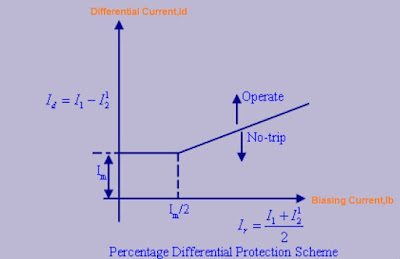
\includegraphics[width=\linewidth]{Proteccion-Diferencial-Porcentual}
    \end{figure}

    

\section{FUSIBLES}

La figura \ref{fig:tiposfusibles} muestra  los principales tipos de fusibles empleados en las redes de distribución.

\begin{figure}[H]
	\centering
	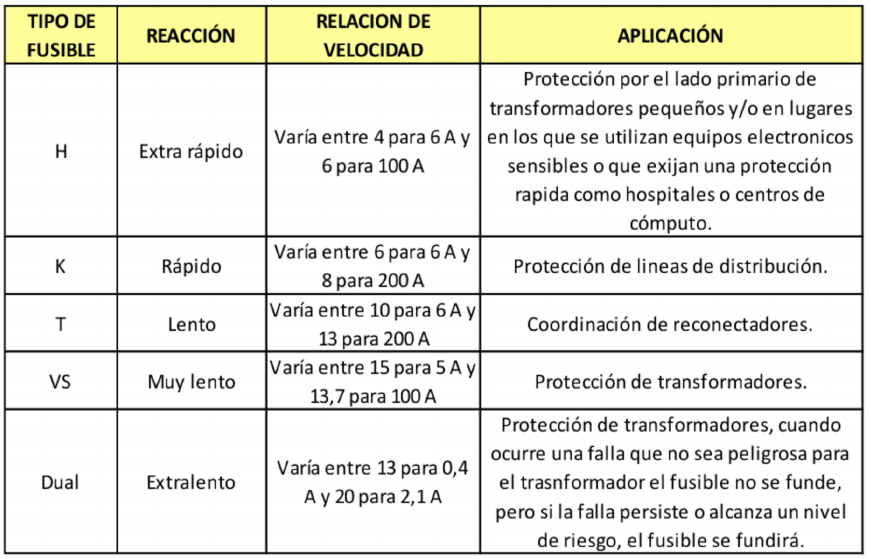
\includegraphics[width=0.7\linewidth]{tipos_fusibles}
	\caption{Tipos de fusibles empleados en media tensión}
	\label{fig:tiposfusibles}
\end{figure}


\chapter{MANTENIMIENTO}


\begin{figure}[H]
  \centering
  % \includegraphics[width=5]{}
  \caption{figura de prueba}
  \label{fig:prueba}
\end{figure}

\chapter{SISTEMAS DE  POTENCIA}

\section{FLUJO DE CARGA}
La potencia activa transmitida por una línea esta dada por la ecuación \ref{eq:1}:

\begin{equation}
  \label{eq:1}
  P=\dfrac{E_{1} \cdot E_{2} \cdot sen\delta } {X}
\end{equation}

En la figura \ref{fig:lineaat} se muestra una línea de transporte de alta tensión donde la impedancia de la línea \textit{$X$} se considera totalmente reactiva y los fasores de tensión  \textbf{$E_{1}$ }y \textbf{$E_{2}$} son las tensiones en la barra del transmisor y del receptor.\\\\

\begin{figure}[H]
  \centering
  
  \caption{Línea de transporte de alta tensión}
  \label{fig:lineaat}
  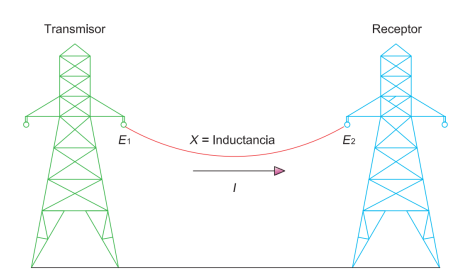
\includegraphics[width=\linewidth]{linea_transporte_AT}
\end{figure}

Entonces se puede obtener los flujos de potencia activa y reactiva
para los siguientes casos \cite{trashorras2015subestaciones}:

\begin{tabular}[H]{|p{0.2\linewidth}|p{0.35\linewidth}|p{0.35\linewidth}|}
  \hline
  CASO & Potencia \textbf{activa} & Potencia \textbf{reactiva}\\\hline
  Distintas magnitud de tensiones  y desfasadas. figura \ref{fig:caso1}  & El flujo de potencia activa siempre es de la tensión adelantada a la  retrasada& La linea absorve reactiva de ambos extremos\\\hline
  Distintas tensiones pero en fase. figura \ref{fig:caso2} & cero&la potencia fluye del nodo  de mayor tensión al de menor tensión y la línea absorve potencia reactiva  \\\hline
  Iguales tensiones pero desfasadas. figura \ref{fig:caso3}  &la línea transporta potencia activa proporcional a las perdidas &la línea absorve potencia reactiva de ambos extremos\\\hline
\end{tabular}


\begin{figure}[H]
  \centering
  \caption{Caso 1: esquema de flujo de potencia con tensiones distintas
    desfasadas.}
  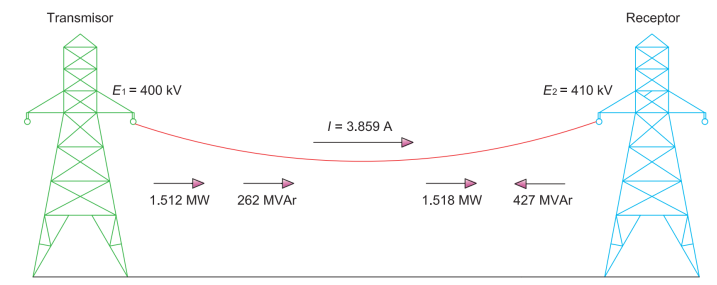
\includegraphics[width=\linewidth]{caso1}
  \label{fig:caso1}
\end{figure}


\begin{figure}[H]
  \centering
  \caption{Caso 2: esquema de flujo de potencia con tensiones distintas en
    fase.}
  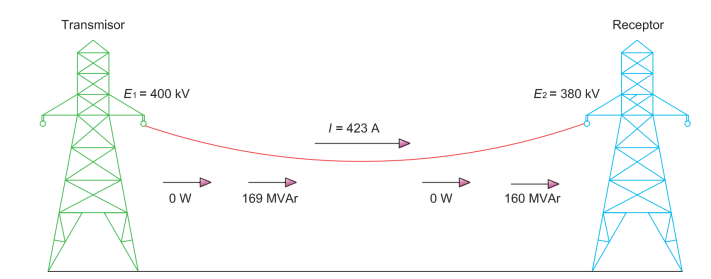
\includegraphics[width=\linewidth]{tensiones_distintas_igual_fase}
  \label{fig:caso2}
\end{figure}

\begin{figure}[H]
  \centering
  \caption{Caso 3: esquema de flujo de potencia con iguales tensiones
    desfasadas.}
  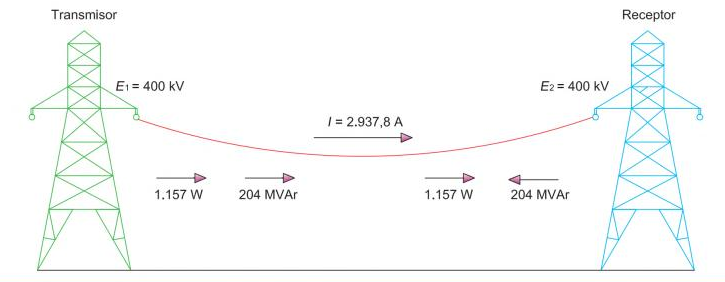
\includegraphics[width=\linewidth]{tensionesigualesdesfasadas}
  \label{fig:caso3}
\end{figure}

\section{CORTOCIRCUITO}

\begin{figure}[H]
  \centering
  \caption{fasores ante un corto circuito hacia adelante y hacia atraz}
  \label{fig:fasores}
  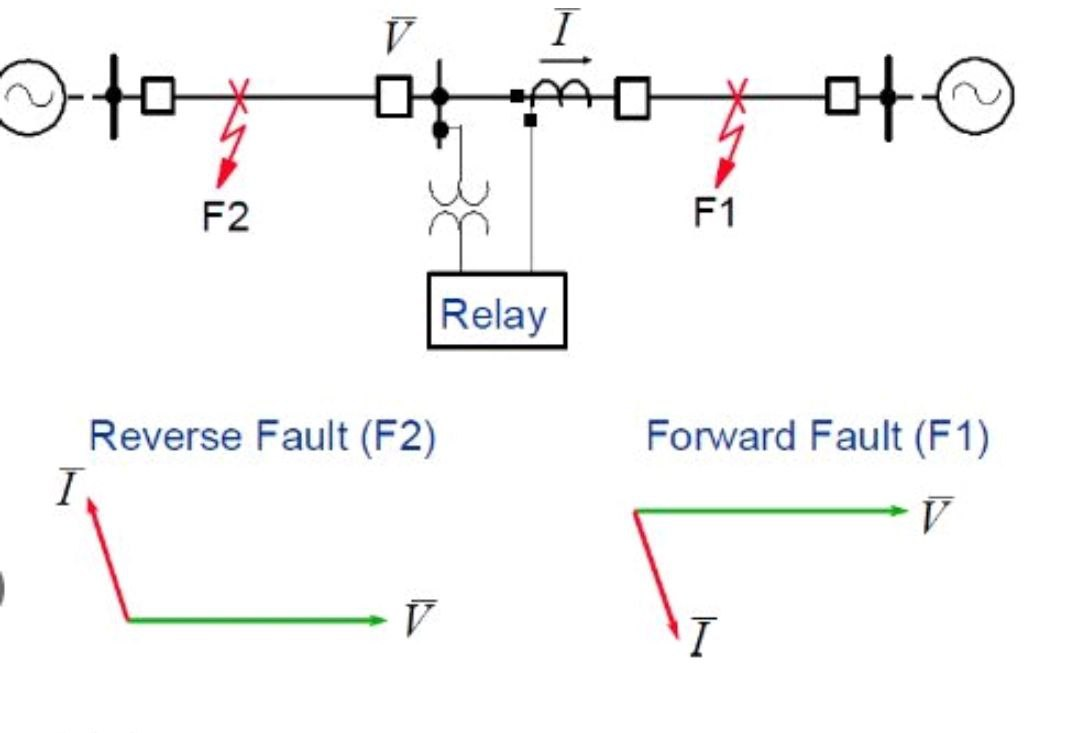
\includegraphics[width=\linewidth]{cortcircuito}
  \end{figure}

\chapter{PLANTAS FOTOVOLTAICAS}

La resolución \cite{CREG-060-2019} establece las normas para operación
de plantas fotovoltáicas, lo  cual implica cambios en los criterios de
ajustes de protecciones, calidad de la potencia ,  control de tensión
y despacho.

La resolución CREG 148 del 2021. Se reportan variables para plantas
solares y fotovoltaicas.\\\\

\begin{itemize}
\item Acuerdos CNO 1521: Calidad de las vairiables reportadas.
\item
\end{itemize}

La generación distribuida  y la auto generación es tratada en la resolución CREG 030 del 2018 y sus limites son los definidos en la figura \ref{fig:gd}.

\begin{figure}[H]
	\centering
	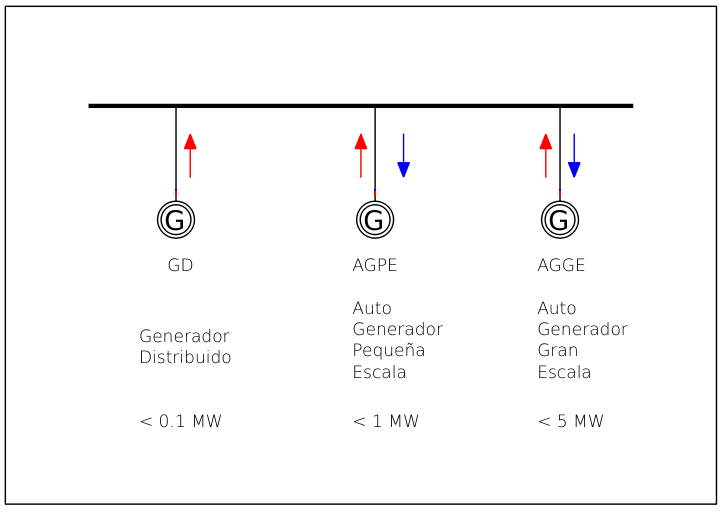
\includegraphics[width=0.7\linewidth]{gd}
	\caption{Capacidad de la auto generación y la generación distribuida}
	\label{fig:gd}
      \end{figure}
      
\chapter{SISTEMA DE GESTIÓN DE CALIDAD}

\chapter{ELEMENTOS DE UNA SUBESTACIÓN}

\section{TRANSFORMADORES}
\subsubsection{POLARIDAD}

La dirección relativa de los voltajes inducidos, que aparecen en los terminales de los devanados secundarios, depende del sentido en que estos terminales se enrollan dentro del núcleo  del transformador. Como los voltajes primario y secundario son inducidos por el mismo flujo mutuo, estos deben estar en la misma dirección. La forma en que aparecerán los voltajes inducidos como se ve desde los terminales del secundario depende de la dirección relativa de los devanados. La polaridad se refiere al orden definido en el que se sacan los terminales del tanque. La polaridad puede definirse como las relaciones vectoriales de voltaje de los cables del transformador extraídos del tanque. Con referencia a la figura \ref{fig:polaridadtransformadores}a, la polaridad es la dirección relativa del voltaje inducido de H1 a H2 en comparación con el de X1 a X2, ambos en el mismo orden.  \cite{POWERSADAS2012}\\\\
Cuando los devanados primarios y secundarios tienen el mismo sentido de arrollamiento se dice que tienen polaridad sustractiva, mientras que si el sentido del devano es opuesto se dice que las polaridades son aditivas.

\begin{figure}[H]
	\centering	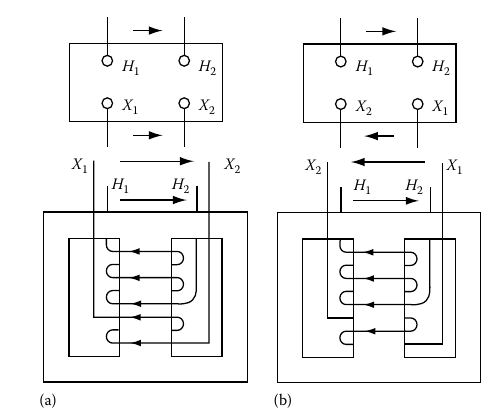
\includegraphics[width=0.7\linewidth]{polaridad_transformadores}
	\caption{Marcas de polaridad a) sustractiva b) aditiva}
	\label{fig:polaridadtransformadores}
\end{figure}

\subsection{Operación en paralelo de transformadores}

Para acoplar dos transformadores en paraleleo se deben tener en cuenta
los siguientes factores \cite{POWERSADAS2012}:

\begin{itemize}
\item La secuencia de fase debe ser la mísma.
\item La polaridad debe ser la misma.
\item La relación de tensiones debe ser la mísma
\item La impedancia de corto circuito debe ser la misma.
\end{itemize}

El reparto de carga en el transformador depende de la diferencia de
las impedancias de los transformadores:

\[ I_{1}= \dfrac{IZ_{2}}{Z_{1}+Z_{2}} \]

\[ I_{2}= \dfrac{IZ_{1}}{Z_{1}+Z_{2}} \]

Donde:

\begin{tabular}{ll}
  $I_{1} y I_{2}$ & Son las corrientes de fase de cada de cada transformador \\
  $I$& es la suma de las corrientes \\
\end{tabular}

\paragraph{Ejemplo}

\begin{figure}[H]
  \centering
  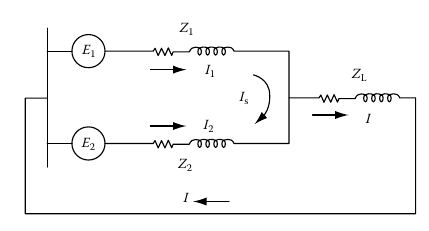
\includegraphics[width=\linewidth]{paralelo_trafo}
  \caption{circuito equivalente de circuito en paralelo}
  \label{fig:paralelo}
\end{figure}
Un transformador  de  10 MVA, 13.8–4.16 kV tiene una resistencia  y una reactancia en por unidad  de 0.005 y 0.05 , respectivamente. Este está en paralelo con un transformador de 5 MVA con la misma relación de transformación, y tiene una reactancia en por unidad de  0.006 y 0.04, respectivamente, calcule como pueden alimentar los dos una carga de 15 MVA con un factor de potencia de 0.8 en atrazo.

Convert Z1 and Z2 on any common MVA base and apply Equations C.14 and C.15. The results are as follows:

10 MVA transformer: S1 1⁄4 9.255 < 37.938
5 MVA transformer: S2 1⁄4 5.749 < 35.208

\section{PUESTA A TIERRA}

La resistencia de puesta a tierra es un indicador que limita directamente la
máxima elevación de potencial, pueden tomarse como referencia los valores máximos de la tabla \ref{tab:valorestierraretie}.

\begin{table}[H]
	\centering
	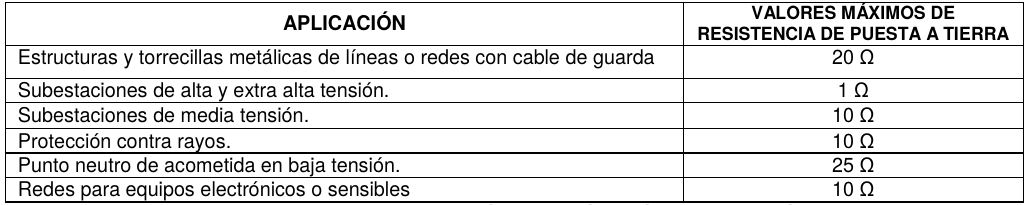
\includegraphics[width=0.7\linewidth]{valores_tierra_retie}
	\caption{Valores de puesta a tierra de acuerdo al RETIE \cite{RETIE2013}}
	\label{tab:valorestierraretie}
\end{table}

La forma como se conecta la tierra y el neutro esta determinado por el régimen de neutro , los cuales pueden ser del tipo TN, TT y TI. En la figura  \ref{fig:tnsystem} muestra los los sistemas  solidamente puestos a tierra. En al figura 

\begin{figure}[H]
	\centering
	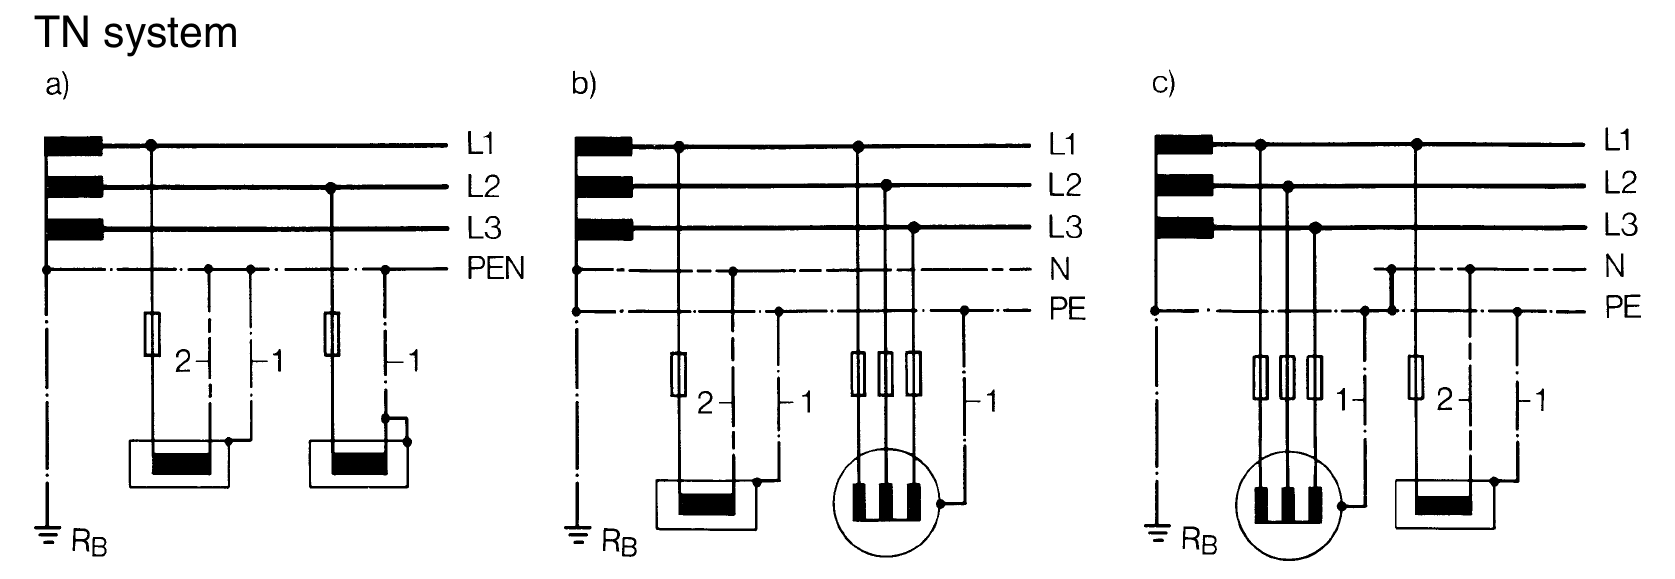
\includegraphics[width=0.9\linewidth]{tnsystem}
	\caption{Sistema TN,  a) TN-C tierra y neutro combinado, b) TN-S tierra neutro separado, TN-CS tierra neutro combinado separado }
	\label{fig:tnsystem}
\end{figure}


\begin{figure}[H]
	\centering
	%\includegraphics[width=0.9\linewidth]{../../../../../../..//home/alejandro/Pictures/tttisystem}
	\caption{Regimen TT y IT}
	\label{fig:tttisystem}
\end{figure}

\begin{table}
	\caption{Coordination of the type of earthing of the systems and protection devices
		}
	\centering
	\begin{tabular}{|c|c|}
		\hline
		Sistema &Dispositivos de protección\\\hline
		TN-S y TN-C-S &sobre corriente  y corrientes de falla\\\hline
		TN-C & sobre corriente \\\hline
		TT & sobrecorriente, corriente de falla\\\hline
		IT & sobrecorriente \\\hline
	\end{tabular}
	
\end{table}


\section{CÁMARAS DE  MEDIA TENSIÓN}
las dimensiones de las cámaras de media tensión son las siguientes (dimensiones en centímetros):\\

\begin{tabular}{|c|c|c|c|}
\hline
Inspección y desviación (0-30°) & 80&100&140 \\\hline 
Cámara de Tiro (T) & 120&230&180 \\\hline
Desviación 2 vías (D2) & 160&160&180\\\hline
Desviación 3 vías (D3) &160&230&180  \\\hline
Desviación 4 vías (D4) & 230&230&180 \\\hline
Maniobra (M) & 300&250&220  \\\hline
Transformación (TR) & 300&250&220  \\\hline
\end{tabular}

 \textbf{Inspección (I).}
Inspección y desviación (0-30°) de redes en media o media y baja tensión, donde solamente existe 1 nivel de conductos en media tensión. Incluye halado y empalme de redes en baja tensión.\\
La distancia máxima entre cámaras es de 60 metros, solo para circuitos en media tensión sin redes baja tensión y 40 metros para circuitos combinados de media y baja tensión.\\\\

\textbf{Tiro (T o TR100)}
Cámara de Tiro (T) para tiro, halado, empalme y desviación (0 – 45o) y transposición de cables para circuitos a 13.2 kV o cámara de inspección TR100 para circuitos a 34.5 kV que sirven de enlace entre subestaciones.\\


\textbf{Desviación 2 vías (D2)} Halado, inspección, empalme y desviación (45°-135°) de redes en media o media y baja tensión. Debe localizarse de acuerdo con la necesidad del proyecto específico.\\\\

\textbf{Desviación 3 vías (D3)}.
Halado, inspección, empalme y desviación (0-135°), 3 direcciones (en T), de redes en media y baja tensión. Debe localizarse sobre las intersecciones de vías en forma de " T " o de acuerdo con las necesidades del proyecto específico.\\\\
\textbf{Desviación 4 vías (D4)}
Halado, inspección, empalme y desviación (0 hasta ± 135°), 4 direcciones (en cruz), de redes en media o media y baja tensión. Debe localizarse en las esquinas,  o de acuerdo con las necesidades del proyecto específico.\\\\
\textbf{Cámara barraje (B2) o TR101}
Cámara B2 para instalar dos barrajes premoldeados a 13.2 kV o cámara TR101 para tiro, halado, empalme o transpocisión de cables de circuitos a 34.5 kV que sirven de enlace entre subestaciones.\\\\
\textbf{Maniobra (M)}
Halado, inspección, empalme y desviación (0-45°), de redes en media o media y baja tensión e instalación de una caja de maniobra (4 a 6 vías), 1 barraje premoldeado de 4 vías y motobomba. Debe localizarse de acuerdo con los datos básicos del proyecto y a la necesidad de equipos de maniobra.

\section{CONDUCTORES}

La capacidad de los conductores

\begin{figure}[H]
  \centering
  \caption{Listado de capacidad de los conductores}
  \label{fig:capacidaddeconductores}
  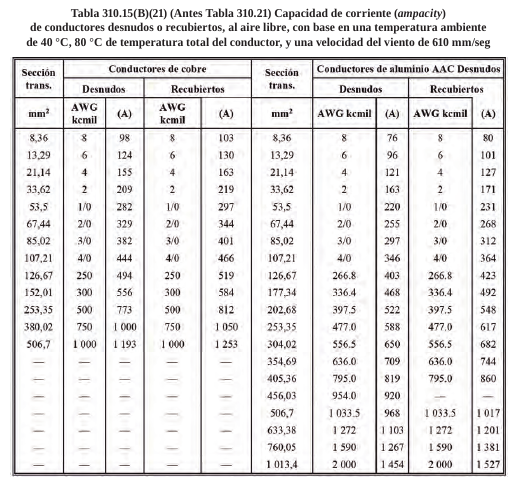
\includegraphics[width=\linewidth]{capacidad_cables_ntc_2050}
\end{figure}

\chapter{MONTAJE, INSTALACIÓN Y PRUEBAS ELÉCTRICAS}

\section{Pararrayos}

La conexión de los descargadores de sobretensiones a los
cortacircuitos se realiza , con conductor de cobre duro desnudo de
21.14 mm2 (4 AWG)Se utilizarán descargadores tipo óxido metálico de
Zinc

\begin{tabular}{|c|c|c|c|}
  \hline
  Parámetro& Unidad& 13.2 kV& 34.5 kV\\\hline
  Tensión& kV& 12& 30\\\hline
  Corriente de descarga&kA&10&10\\\hline
\end{tabular}

\section{TRANSFORMADORES}

En el caso de transformadores usados y o reparados éstos deben cumplir con los siguientes requerimientos para ser instalados:

\begin{enumerate}
	\item Tiempo de uso no mayor a 14 años (para transformadores usados).
	\item Fecha de fabricación posterior a 1985 (para transformadores reparados).
	\item Certificación de la procedencia del equipo.
	\item Certificación de que el equipo no presenta contaminación por bifenilos policlorados – PCB (resolución DG No. 601 de 2002 de CVC).
	\item  Protocolo de pruebas con las siguientes características.
	\begin{itemize}
		\item Datos de placa
		\item  Prueba de relación de transformación.
		\item  Prueba de resistencia de aislamiento
		\item  Prueba de resistencia de devanados y pruebas de pérdidas (vacío y carga).
	\end{itemize}
      \end{enumerate}

      \section{Pruebas a equipos eléctricos}

\begin{figure}[H]
	\centering
	\caption{Pruebas sobre transformadores}
	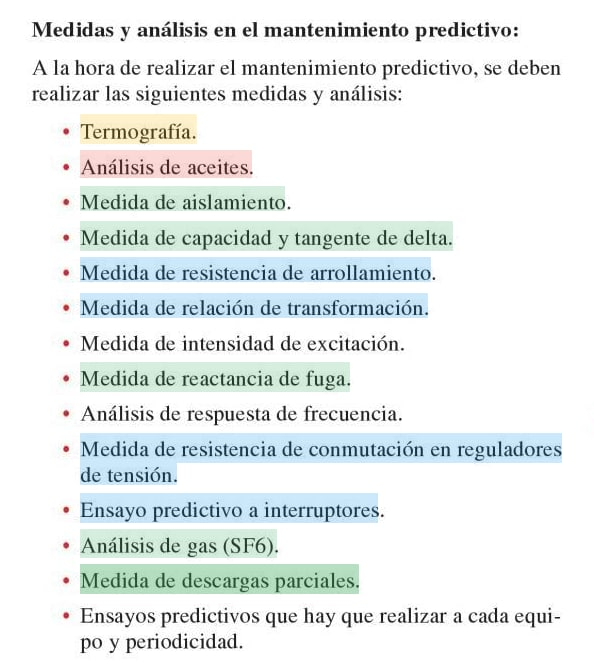
\includegraphics[width=0.7\linewidth]{pruebas}
	\label{fig:pruebas}
\end{figure}

\chapter{COMUNICACIONES Y CONFIGURACIONES}

\section{Acuerdos y regulación aplicable a las comunicaciones}

\subsection{Regulación}
La regulación aplicable a las comunicaciones es la siguiente:

\begin{itemize}
\item CREG 025 – 1995: Código de Redes, como parte del Reglamento de Operación del Sistema Interconectado Nacional
\item CREG 080 - 1999: Funciones de planeación, coordinación supervisión y control entre el Centro Nacional de Despacho (CND) y los agentes del SIN
\item CREG 060 - 2019: Reglamento de Operación para permitir la conexión y operación de plantas solares fotovoltaicas y eólicas en el SIN
\item CREG 148 - 2021: Conexión y operación de plantas solares fotovoltaicas y eólicas en el SDL con capacidad efectiva neta o potencia máxima declarada igual o mayor a 5 MW
\end{itemize}

\subsection{Acuerdos}

los acuerdos vigentes con relación a las comunicaciones son :

\begin{itemize}
\item 1411: Por el cual se aprueban los procedimientos y los indicadores relacionados con la Supervisión del SIN
\item 1428: Requisitos para la Prestación del Servicio de Regulación Secundaria de Frecuencia – AGC
\item 1525: Por el cual se aprueban los requisitos de la supervisión de las variables eléctricas de las plantas solares fotovoltaicas y eólicas en el SDL con capacidad efectiva neta o potencia máxima declarada igual o mayor a 5 MW
\item 1612: Puesta en operación de proyectos de transmisión que incluyan activos de uso del STN, STR, SDL y recursos de Generación
  \end{itemize}


Los protocolos de comunicaciones empleados en los sistemas eléctricos son los que se muestran en la figura \ref{fig:protocoloscomunicacion} de lo que se destaca la comunicación entre el \ac{OR} y el \ac{CND}, en que los OR se comunican con el \ac{CND} mediante el protocolo \textbf{ICCP} (\textit{Inter Control Center Communication Protocol}).

\begin{figure}[H]
  \centering
  \caption{Protocolos de comunicación en sistemas ecléctico}
  \label{fig:protocoloscomunicacion}
  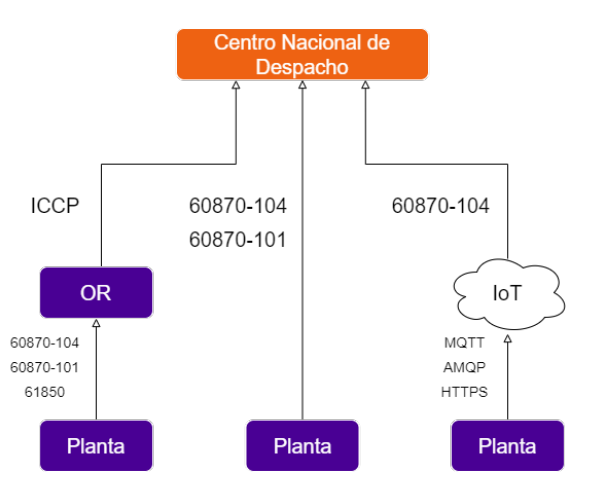
\includegraphics[width=0.5\linewidth]{protocolos_comunicacion}
\end{figure}

El protocol ICCP  es basado en el concepto cliente servidor. Este protocolo se desarrolla en la capa 7 del modelo OSI. Todas las transferencias de datos se originan con una solicitud de un centro de control (el cliente) a otro centro de control que posee y administra los datos (el servidor). \texttt{Por ejemplo, si una aplicación del Centro de Control X necesita datos de la base de datos SCADA de Centro de Control Y, la aplicación Control Center X, que actúa como cliente, podría solicitar que Control Center Y, que actúa como servidor, envíe los datos en las condiciones especificadas por el cliente}.\\

\begin{figure}[H]
  \caption{Comunicación en la capa 7 para el protocolo ICCP}
  \label{fig:capa7iccp}
  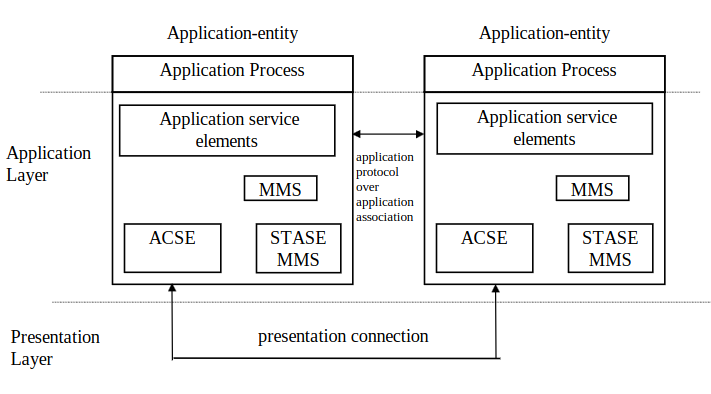
\includegraphics[width=\linewidth]{capas_iccp}
\end{figure}


El Association Control Service Element (ACSE) es un mecanismo utilizado por el protocolo ICCP (Inter-Control Center Communications Protocol) para el establecimiento de asociaciones lógicas entre un cliente y múltiples centros de control servidores\\\\
% Existen varios servicios proporcionados en \textbf{ICCP} para realizar transferencias de datos, según el tipo de solicitud. Por ejemplo, si el cliente realiza una solicitud única, los datos se devolverán como un respuesta a la solicitud. Sin embargo, si el cliente solicita la transferencia periódica de datos o la transferencia de datos solo cuando cambian, entonces el cliente establecerá primero el informe. El servidor (es decir, especificar condiciones de informes como la periodicidad de las transferencias periódicas u otras condiciones desencadenantes como el informe por excepción únicamente), y el servidor luego enviará los datos como un informe no solicitado siempre que se cumplan las condiciones de informe.\\\\


  \section{Informe de superación y enlaces CND}

  En cada punto a supervisar el valor será de 100\% si está supervisado, o 0\% si no está supervisado. Porcentaje de tiempo en que el Punto a Supervisar llega al sistema SCADA del CND. La meta CNO: 95\%, pero la meta del la CREG es 97 \%,  con periodicidad semanal. Para realizar este reporte se utiliza la plataforma GAO.


  
  De acuerdo a la resolución \textbf{CREG 083 de 1999} Por cada evento que se registre se debe enviar la fecha y hora con \textit{resolución de un (1) ms}, la identificación del elemento que cambió de estado y el estado. final del dispositivo.\\\\


  \section{Automatización de Subestaciones}

En la automatización de subestaciones,  se reconocen  tres componentes dentro de la red de comunicación:

\begin{itemize}
\item nivel de estación (\textit{station bus}) se caracteriza por comunicar los relay (IDE)  con el gateway,  con velocidades de 10 a 1GB.
\item nivel de proceso (\textit{process bus}) se caracteriza por comunicar las MU (\textit{Merging Unit}) ó los concentradores de medidas con los relés de la estación.
\item nivel de bahía
\end{itemize}

\begin{figure}[H]
  \centering
  
  \caption{Estructura de redes de comunicación del protocolo IEC61850}
  \label{fig:iec61850}
  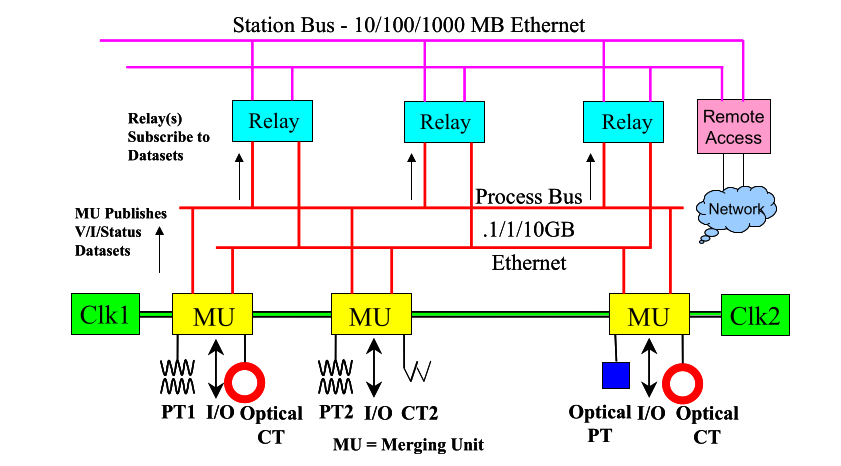
\includegraphics[width=\linewidth]{iec61850}
\end{figure}



\subsection{Modelo de Datos IEC 61850}

El modelo de datos IEC 61850 es una representación jerárquica de la información dentro de un IED (Dispositivo Electrónico Inteligente). Su propósito es estandarizar la comunicación y el intercambio de información en sistemas de automatización de subestaciones.

\begin{figure}[H]
  \centering
  \caption{Estructura IEC61850}
  \label{fig:iec61850}
  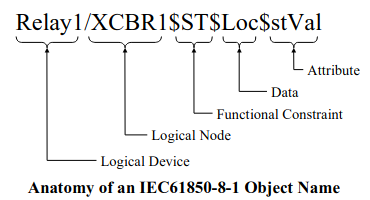
\includegraphics[width=0.5\linewidth]{anatomia_iec}
\end{figure}

\begin{figure}[H]
  \centering
  \caption{Estructura IEC61850 esquema gráfico}
  \label{fig:iec61850_ln}
  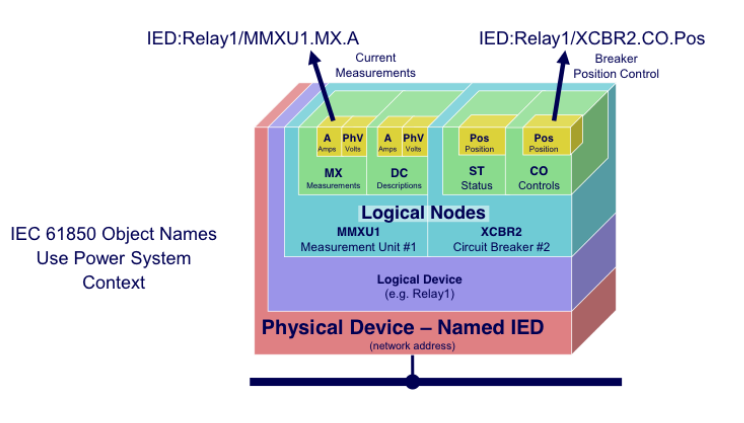
\includegraphics[width=0.7\linewidth]{LNs}
\end{figure}

\paragraph{Estructura Jerárquica}

\begin{enumerate}
\item     Dispositivo Lógico (Logical Device): El nivel superior del modelo, una colección de múltiples nodos lógicos.
    
\item Nodo Lógico (Logical Node): Modela las  aplicaciones y contienen objetos de datos.
    
\item Objeto de Datos (Data Object): O data de acuerdo a la figura \ref{fig:iec61850} están dentro de los nodos lógicos, su estructura está definida por la Clase de Datos.
    
\item Atributo de Datos (Data Attribute): es donde se encuentran los valores de los data objects.
  \end{enumerate}

\subsubsection{ Dispositivo Lógico (Logical Device)}

Estan definidos principalmente por el fabricante más que por la norma IEC 61850 y hacen referencia a los IDEs. De acuerdo a la figura \ref{fig:iec61850} hace referencia a Relay1.

\subsubsection{Nodo Lógico (Logical Node - LN)}

Es el elementos clave para modelar los elementos que componen los sistemas de comunicación, protecciones y automatización (ej. el elemento de la protección de distancia, interfaz a un seccionador).\\\\
Los nombres son estandarizados con cuatro caracteres. El primer carácter indica el grupo  (ej. P para protección, X para los equipos de maniobra). Los nodos se agrupan en grupos funcionales:

\begin{table}[H]
  \centering
  \begin{tabular}{|l | p{0.2\linewidth} |p{0.4\linewidth}|}
    \hline
    Grupo funcional & Designación & Nodos típicos \\\hline
    System & Lxxx & \textbf{LLN0} (Datos de placa del IDE) \\\hline
    Automatic Control & Axxx & \textbf{ATCC} (Cambiador de tomas) \\\hline
    Control & Cxxx & \textbf{CSWI}  (Control de switches)  \\\hline
    Generic Functions & Fxxx & \textbf{FSCH} (funciones programadas) \\\hline
    Interfacing and Archiving & Ixxx & IHMI (representa el sistema SCADA) \\\hline
    Metering  and measurements & Mxxx & MMXU (medidas voltajes corrientes  o frecuencias) \\\hline
    Protection & Pxxx & \textbf{PDIS} (protección de distancia) \textbf{PTUV} (protección de bajo voltaje) \textbf{PDIR} (protección direccional) \textbf{PIOC} (protección de sobre corriente)\\\hline

    Power Quality & Qxxx & \\\hline
    Supervision & Sxxx & \textbf{SLTC} (supervición del OLTC) \textbf{SSWI} (supervición de switches) \textbf{SPTR} (supervición a transformadores de potencia) \\\hline

    Transformador de instrumento & Txxx  & \textbf{TCTR} (transformadores de corriente) \textbf{TVTR} (transformadores de voltaje) \\\hline

    Switchgear & Sxxx & \textbf{XCBR} (interruptor) \textbf{XSWI} (seccionador) \\\hline

    
    \end{tabular}
  \end{table}

  \begin{figure}[H]
  \centering
  \caption{Restricción protocolo IEC61850}
  \label{fig:iec61850resticcion}
  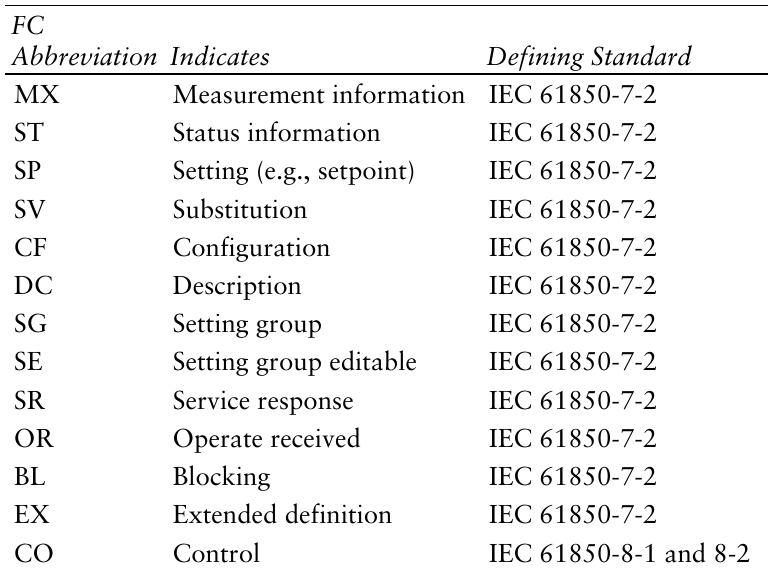
\includegraphics[width=\linewidth]{restricciones}
\end{figure}



\subsubsection{Objeto de Datos (Data Object - DO)}

Componente de un Nodo Lógico. Su estructura y los atributos de datos disponibles están definidos por la Clase de Datos Común (CDC).Un objeto de datos puede tener múltiples atributos de datos. También puede contener sub-objetos de datos (que a su vez son de otras Clases de Datos Comunes).\\\\
Ejemplo:\\
El objeto de datos POS (posición de un interruptor) es de la Clase de Datos Común DPC (Double Point Control).\\\\
    Especificación: Definidos en las partes 7-4, 7-410 y 7-420 del estándar junto con los Nodos Lógicos. Incluyen un nombre, referencia a la CDC, explicación corta e indicación de obligatoriedad/opcionalidad.

\subsubsection{Clase de Datos Común (Common Data Class - CDC)}

    Definición: Una definición de tipo estructurado que define qué atributos de datos están disponibles para un objeto de datos.
    Función: Determina la estructura de un objeto de datos.
    Grupos: Agrupados según sus características principales (ej. SPS para estado de un solo punto, MV para valores medidos, DPC para control de doble punto).
    Especificación: Definidas en la parte 7-3 del estándar. La especificación incluye una lista de atributos de datos, el tipo de atributo (básico o clase de atributo construida), restricción de función, condición de presencia y posibles rangos de valores.
    Ejemplo: INS es una CDC para información de estado de enteros; DPC es una CDC para control de doble punto.

\subsubsection{Atributo de Datos (Data Attribute - DA)}

    Definición: Las hojas de la jerarquía del modelo de datos donde se encuentran los valores.
    Tipos:Tipo Básico (Basic Type): Tipos de datos fundamentales (ej. entero de 32 bits sin signo, punto flotante). Definidos en la parte 7-2.
    Clase de Atributo Construida (Constructed Attribute Class - CAC): Atributos de datos que tienen una estructura interna, es decir, están compuestos por otros sub-atributos de datos (ej. Quality, Vector, AnalogValue, Timestamp).
    Restricciones de Función (Function Constraints - FC): Utilizadas para clasificar los atributos de datos según su propósito. Ejemplos:
    ST: Atributos de estado.
    CF: Atributos de configuración.
    SV: Atributos relacionados con sustitución.
    SP: Atributos de punto de ajuste (settings).
    Contenido: Los atributos de datos pueden ser de un tipo básico o tener niveles jerárquicos adicionales a través de Clases de Atributo Construidas hasta llegar a los componentes primitivos.

    \subsubsection{Clase de Atributo Construida (Constructed Attribute Class - CAC)}
    

    Definición: Un tipo de atributo de datos que posee una estructura interna, es decir, se compone de otros sub-atributos.
    Ejemplos: Quality (calidad de la información), Timestamp (marca de tiempo), Vector (magnitud y ángulo).
    Especificación: Definidas en la parte 7-3 del estándar.

Relación entre los Elementos y las Partes del Estándar

    Parte 7-4 / 7-410 / 7-420: Definen las clases de Nodos Lógicos, su semántica y la estructura en términos de Objetos de Datos, incluyendo nombres, descripciones semánticas y tipos.
    Parte 7-3: Define todas las Clases de Datos Comunes (CDCs) con su estructura en términos de Atributos de Datos (nombres, semántica, tipo). También define las Clases de Atributo Construidas (CACs).
    Parte 7-2: Especifica los tipos básicos y los tipos ACSI comunes.


    La configuración en el estándar IEC 61850 se basa en el uso de **archivos XML** a través del **Lenguaje de Descripción de Configuración de Subestaciones (SCL)**, definido en la parte 6 de la norma [1-6]. El SCL es la parte más importante de la serie IEC 61850 para el diseño de sistemas, ya que todo el proceso de ingeniería se puede apoyar en este lenguaje [2].

Los archivos SCL contienen información crítica del sistema y son fundamentales para el proceso de ingeniería, desde la especificación hasta el despliegue del sistema [3, 5, 7]. Se utilizan para describir las capacidades de los IEDs, el diseño del sistema y la configuración de la comunicación [3, 5, 8-11].


\subsection{Tipos de archivos }

Los principales tipos de archivo SCL empleados en la configuración de 61850 son:

\begin{enumerate}

\item {\textbf{SSD} (\textit{System Specification Description})}:Son el \textit{punto de partida inicial} en el proceso de ingeniería. Proporcionan información sobre la \textit{topología planificada} y los nodos lógicos (LN) requeridos para el sistema.

\item{\textbf{ICD} (\textit{IED Capability Description})}: Describen las capacidades genéricas de un Dispositivo Electrónico Inteligente (IED) específico. Son proporcionados por el fabricante y describen el modelo de datos y las capacidades de comunicación del dispositivo. Contienen una sección IED para el dispositivo cuyas capacidades representa. Antes de ser configurado, el nombre del IED en este archivo es típicamente "TEMPLATE".

\item {\textbf{IID} (\textit{Instantiated IED Description})}: Representan la \textit{funcionalidad de un archivo ICD parcialmente configurado}. En este archivo, el nombre del IED ya no es "TEMPLATE", sino que refleja el rol específico del IED en un esquema estándar.

\item{\textbf{CID} (\textit{Configured IED Description})}: Son archivos de configuración específicos.

\item{\textbf{SCD} (\textit{Substation Configuration Description})}: Son el \textit{resultado final del proceso de configuración} del sistema. Contienen toda la información necesaria para configurar un sistema de automatización de subestaciones . Pueden ser utilizados para una variedad de aplicaciones y son clave para la automatización y la puesta en marcha de los sistemas IEC 61850.

\item {\textbf{SIED} (\textit{System Interface Exchange Description})}:Se utilizan para el intercambio de datos entre herramientas de configuración de sistemas para diferentes proyectos de subestaciones. Son importantes para establecer comunicaciones entre subestaciones, fijando referencias de objetos de origen ya definidas y especificando nuevas conexiones de interfaz entre proyectos.

\end{enumerate}

Además de los archivos SCL, se utilizan otros tipos de archivos en contextos relacionados:

\paragraph{Archivos COMTRADE}: Se utilizan para el \textit{registro de perturbaciones} y para la grabación de perturbaciones basada en sincronofasores. Estos archivos son generados por los nodos lógicos relacionados con la protección.


\subsection{Protocolos empleados en IEC 61850}

En la figura \ref{fig:protocolosiec61850} se muestra la relación de los protocolos empleados en el estandard IEC 61850 y su relación con el modelo OSI.

\begin{figure}[H]
      \centering
      \caption{protocolos empleados en IEC 61850}
      \label{fig:protocolosiec61850}
      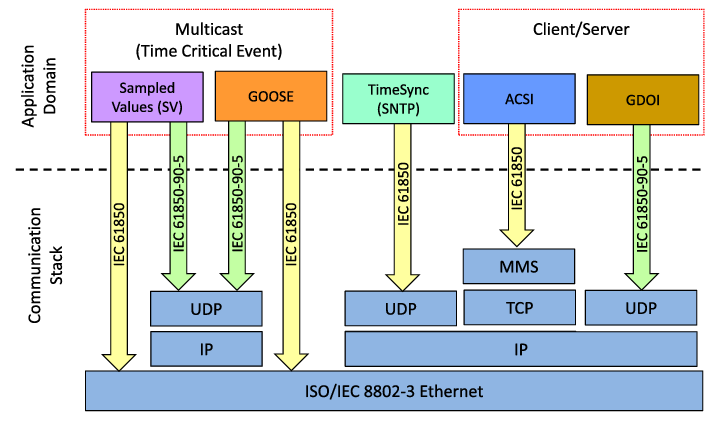
\includegraphics[width=0.7\linewidth]{cliente_servidor_61850}
    \end{figure}


\subsection{Ejemplo de aplicación para el área de protecciones}

    En el siguiete ejemplo correlacionado al área de protecciones se describiran los nodos lógicos que interactuan en la protección de una central de generación, para lo cual se toma como el diagrama de la figura \ref{fig:centralgen}.

    \begin{figure}[H]
      \centering
      \caption{diagrama de la central de generación del ejemplo \thesubsection}
      \label{fig:centralgen}
      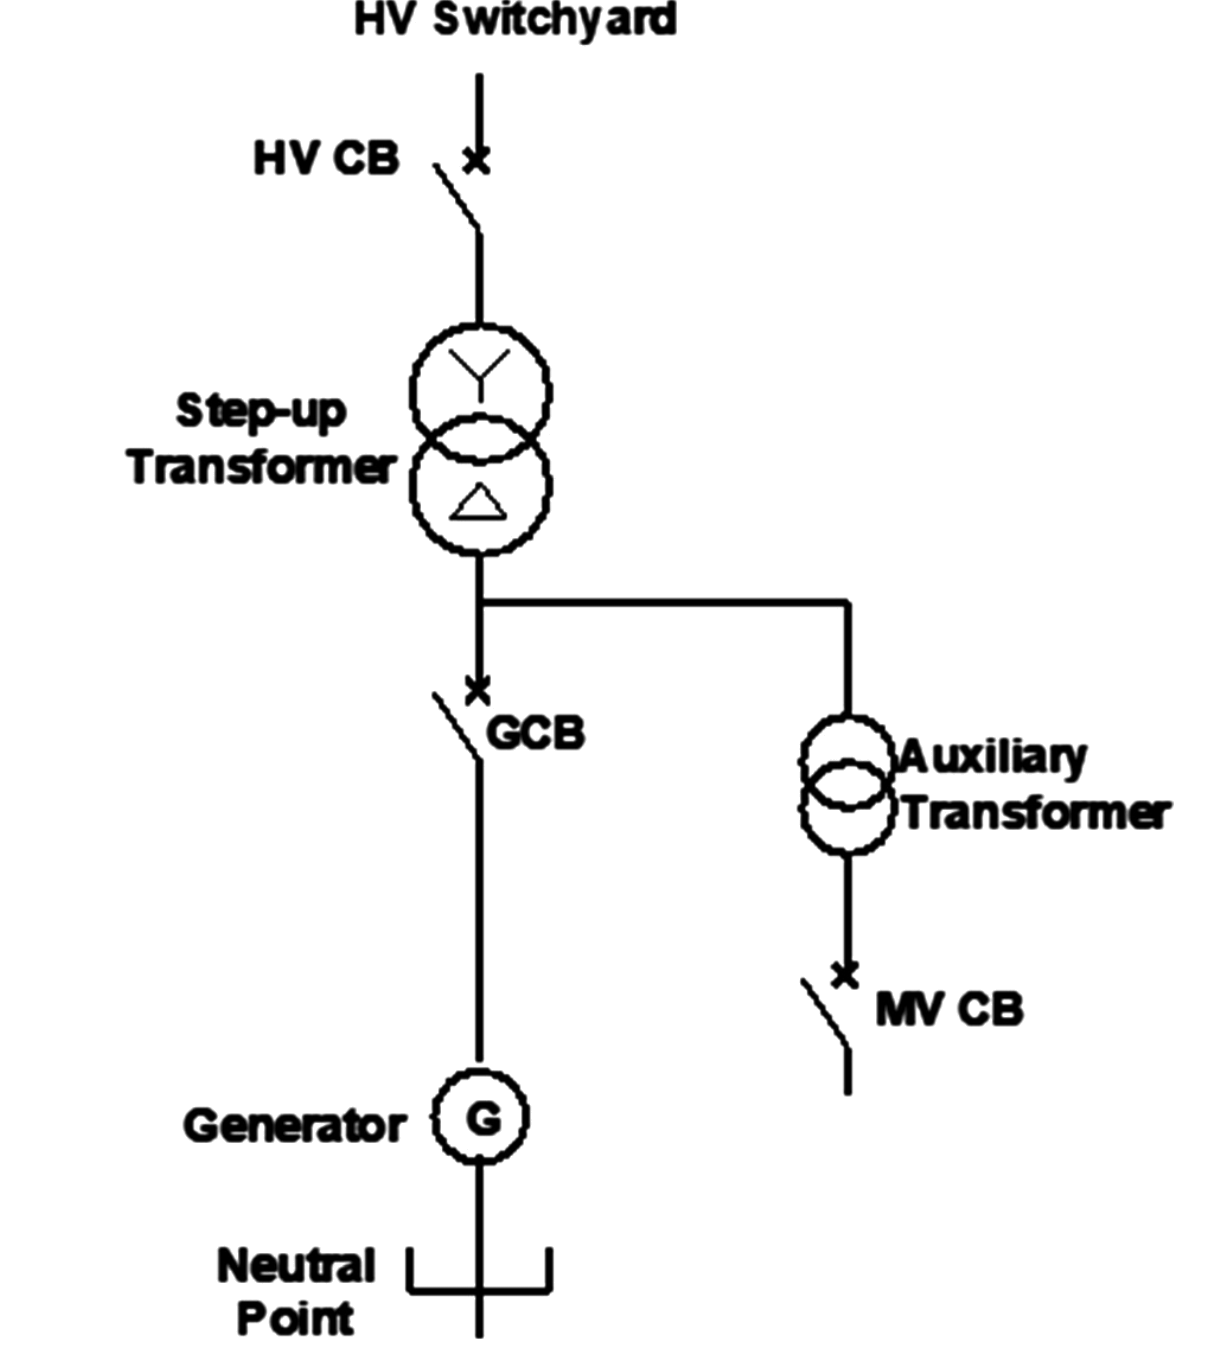
\includegraphics[width=0.7\linewidth]{generador}
    \end{figure}


    \begin{figure}[H]
      \centering
      \caption{nodos lógicos de la central de generación del ejemplo \thesubsection}
      \label{fig:nlcentral}
      \includegraphics[width=0.7\linewidth]{nl_generador}
    \end{figure}    

    \begin{figure}[H]
      \centering
      \caption{tabla nodos logicos de la central de generación}
      \label{fig:tnlcentral}
      \includegraphics[width=0.7\linewidth]{t_nl_generador}
    \end{figure}    
    
    \subsection{Ejemplo para el área de generación}
De acuerdo a lo realizado en \cite{salazar2017},  donde se realiza la estructura de  los nodos lógicos del IEC 61850



    
\subsection{Quiz (10 Preguntas de Respuesta Corta)}

Instrucciones: Responda cada pregunta con 2-3 oraciones.

\begin{enumerate}
\item ¿Cuál es el propósito principal de un Dispositivo Lógico en el modelo de datos IEC 61850 y quién lo define típicamente?
\item Describa qué es un Nodo Lógico y por qué se considera un elemento clave en el modelo.
\item Explique la relación entre un Objeto de Datos y una Clase de Datos Común.
\item ¿Qué son las "hojas" de la jerarquía del modelo de datos IEC 61850 y qué se encuentra en ellas?
\item Diferencie entre un Tipo Básico y una Clase de Atributo Construida en el contexto de los Atributos de Datos.
\item Mencione dos ejemplos de Grupos de Nodos Lógicos y el propósito de esta agrupación.
\item ¿Qué información se utiliza para clasificar los Atributos de Datos según su propósito, y dé un ejemplo?
\item En la especificación de un Nodo Lógico, ¿qué indican las marcas "M" y "O" junto a los Objetos de Datos?
\item ¿Qué parte del estándar IEC 61850 define las Clases de Datos Comunes y qué tipo de información incluyen estas definiciones?
\item Explique cómo un Objeto de Datos puede tener una estructura jerárquica más allá de sus atributos de datos directos.
  \end{enumerate}

Clave de Respuestas del Quiz

\begin{itemize}
\item El propósito principal de un Dispositivo Lógico es agrupar Nodos Lógicos para funciones específicas, como protección o control, y para la gestión del comportamiento del dispositivo. Estos no son definidos por el estándar, sino típicamente por el fabricante del IED.
\item Un Nodo Lógico es un elemento clave para modelar funciones de aplicación, representando una funcionalidad fraccional (ej. un elemento de protección o una interfaz a un interruptor). Contiene todos los datos relacionados con esa función, estandarizando su representación.
\item Un Objeto de Datos es un componente de un Nodo Lógico, y su estructura, es decir, qué Atributos de Datos están disponibles, está completamente definida por su Clase de Datos Común. La CDC actúa como una plantilla o tipo estructurado para el Objeto de Datos.
\item Las "hojas" de la jerarquía del modelo de datos IEC 61850 son los Atributos de Datos. Es en estos atributos donde finalmente se encuentran los valores de la información modelada, ya sea directamente o dentro de estructuras anidadas.
\item Un Tipo Básico es un tipo de dato fundamental y primitivo (ej. entero, punto flotante) que no tiene una estructura interna adicional. Una Clase de Atributo Construida, en cambio, es un tipo de atributo de datos que posee una estructura interna y se compone de otros sub-atributos (ej. Quality, Timestamp).
\item Dos ejemplos de Grupos de Nodos Lógicos son "Protección" (ej. PDIF para protección diferencial) y "Aparamenta" (ej. XSWI para interruptor). Esta agrupación facilita el manejo y la comprensión de las funcionalidades estandarizadas.
\item Las Restricciones de Función (Function Constraints - FC) se utilizan para clasificar los Atributos de Datos según su propósito. Por ejemplo, ST identifica atributos de estado, mientras que CF identifica atributos de configuración.
\item En la especificación de un Nodo Lógico, la indicación "M" (obligatorio) significa que el Objeto de Datos debe estar presente en la implementación de ese Nodo Lógico. La "O" (opcional) indica que su presencia es discrecional.
\item La Parte 7-3 del estándar IEC 61850 define las Clases de Datos Comunes. Estas definiciones incluyen una lista de atributos de datos, su nombre, semántica, tipo, la restricción de función y la condición de presencia.
\item Un Objeto de Datos puede tener una estructura jerárquica adicional si una de sus Clases de Datos Comunes se refiere a otros objetos de datos, que a su vez son de otras Clases de Datos Comunes. Un ejemplo es la CDC Y para mediciones trifásicas, que contiene sub-objetos para cada fase (ej. Phase A, Phase B, Phase C) de tipo CMV.
\end{itemize}

Preguntas de Formato Ensayo (No se proporcionan respuestas)

\begin{enumerate}
\item Analice cómo la estructura jerárquica del modelo de datos IEC 61850 (Dispositivos Lógicos, Nodos Lógicos, Objetos de Datos, Atributos de Datos) contribuye a la estandarización y modularidad de la comunicación en los sistemas de automatización de subestaciones.
\item Compare y contraste el papel de las Clases de Datos Comunes (CDCs) y las Clases de Atributos Construidas (CACs) en la definición de la estructura y el tipo de los datos dentro del modelo IEC 61850. Incluya ejemplos para ilustrar su explicación.
\item Explique cómo las diferentes partes del estándar IEC 61850 (7-2, 7-3, 7-4/7-410/7-420) colaboran para proporcionar una definición completa y coherente de los elementos del modelo de datos.
\item Discuta la importancia de las Restricciones de Función (Function Constraints) y la indicación de obligatoriedad/opcionalidad en la especificación de los Objetos de Datos y Atributos de Datos para la flexibilidad y la correcta interpretación del modelo.
\item Utilizando el ejemplo del Objeto de Datos POS (posición de un interruptor), describa cómo se modelan tanto la información operativa como la no operativa (ej. configuración, sustitución) dentro de un mismo Objeto de Datos y la relevancia de los Atributos de Datos para ello.
\end{enumerate}


Glosario de Términos Clave

\begin{itemize}
\item ACSI (Abstract Communication Service Interface): Interfaz de Servicio de Comunicación Abstracta. Parte del estándar IEC 61850 que define los servicios abstractos para la comunicación entre IEDs.
\item Atributo de Datos (Data Attribute - DA): El elemento más básico del modelo de datos, donde se encuentra el valor de la información. Puede ser de un tipo básico o una clase de atributo construida.
\item Clase de Atributo Construida (Constructed Attribute Class - CAC): Un tipo de atributo de datos que tiene una estructura interna, es decir, se compone de otros sub-atributos (ej. Quality, Timestamp).
\item Clase de Datos Común (Common Data Class - CDC): Una definición de tipo estructurado que define la lista de atributos de datos disponibles para un objeto de datos, determinando su estructura.
\item Dispositivo Lógico (Logical Device): El nivel superior de la jerarquía del modelo de datos, una colección de Nodos Lógicos que agrupa funcionalidades.
\item IEC 61850: Un estándar internacional para la comunicación en subestaciones eléctricas y, por extensión, en sistemas de automatización de la energía, que define un modelo de datos orientado a objetos.
\item IED (Intelligent Electronic Device): Dispositivo Electrónico Inteligente. Un dispositivo basado en microprocesador utilizado en sistemas de energía, como relés de protección, RTUs y controladores.
\item Nodo Lógico (Logical Node - LN): Elemento clave del modelo de datos que representa una función de aplicación específica (ej. un relé de protección, un interruptor) y contiene los datos asociados.
  
\item Objeto de Datos (Data Object - DO): Un componente de un Nodo Lógico cuya estructura está definida por una Clase de Datos Común. Puede contener múltiples atributos de datos.
  \item Restricción de Función (Function Constraint - FC): Un clasificador utilizado para categorizar los atributos de datos según su propósito (ej. ST para estado, CF para configuración).
  \item Servidor IEC 61850: Un componente de un IED que expone el modelo de datos IEC 61850 a otros dispositivos o sistemas.
  \item Tipo Básico (Basic Type): Un tipo de dato primitivo y fundamental (ej. entero de 32 bits, punto flotante) que no posee una estructura interna.
\end{itemize}

    
\chapter{PROCESO DE CONEXIÓN}

\section{Conexión de usuarios}

Los proyectos se pueden clasificar de acuerdo a la resolución CREG 075
del 2021 en tipo 1 y tipo 2 , como lo muestra la figura
\ref{fig:tipoproyecto}. Estos no incluyen los proyectos del tipo
\ac{FNCER} citados en la resolucion CEG 030 del 2018.


\begin{figure}[H]
  \centering \includegraphics[width=1\linewidth]{tipoproyecto}
  \caption{Tipos de proyecto de acuerdo a resolución CREG 075 del
    2021}
  \label{fig:tipoproyecto}
\end{figure}

    \section{ENTRADA EN OPERACIÓN COMERCIAL}

    El procedimiento guía y los plazos aclaratorios no previstos en la regulación para la entrada en operación de plantas al SIN de Activos dei Sistema de Transmisión Nacional - STN del Sistema de Transmisión Regional - STR - y de Activos de conexión al STN,  se ,muestra en el acuerdo 646 del 2013, como se muestra en la figura \ref{fig:plazo646}.

    \begin{figure}[H]
      \caption{Plazos Acuerdo CNO 646 de 2013}
      \label{fig:plazo646}
      \includegraphics[width=\linewidth]{plazo_cno}
      \end{figure}


\chapter{SEGURIDAD EN EL TRABAJO}
Al realizar trabajo de campo sobre o al rededor de redes eléctricas de distribución como medida de protección deben usarse las distancias de seguridad \cite{RETIE2013}.\\\\

Las distancias de seguridad pueden clasificarse según su uso en :

\begin{itemize}
\item Distancias en construcciones.
\item Distancias en vías.
\item Distancias en zonas verdes ( cultivos, pastos, bosques).
\item Distancias en ríos y fuentes de agua.
\item Distancias entre conductores en la misma estructura.
\item Distancias de personal al realizar mantenimiento.
\end{itemize}

Estas distancias a su vez se subdividen de acuerdo a otros criterios como el nivel de tensión y los tipos de aislamiento de los conductores energizados.

\section{TRABAJOS CON TENSIÓN}

Todo trabajo en circuitos energizados de más de 450 voltios debe hacerse con un grupo de trabajo de al menos dos (2) personas. Los grupos de trabajos que realicen labores en circuitos por encima de 1000 V deben contar con al menos dos (2) operarios y un (1) jefe que coordine y supervise las labores estando atento del trabajo del grupo para controlar cualquier riesgo que los pueda afectar en
el desarrollo del trabajo.  \cite{RETIE2013}\\\\

Los métodos de trabajo más comunes, para operar con tensión son: \cite{RETIE2013}:

\begin{enumerate}
	\item Trabajo a distancia: En este método, el operario ejecuta
          el trabajo con la ayuda de herramientas montadas en el
          extremo de pértigas aislantes \ref{fig:trabajoadistancia}.
	\item Trabajo a contacto: En este método, el operario se aísla
          del conductor en el que trabaja y de los elementos tomados
          como masa por medio de elementos de protección personal,
          dispositivos y equipos aislantes \ref{fig:trabajocontacto}.
	\item Trabajo a potencial: En el cual el operario queda al
          potencial de la línea de transmisión en la cual trabaja,
          mediante vestuario conductivo \ref{fig:trabajoapotencial}.
        \end{enumerate}

        \begin{figure}[H]
          \centering
          \caption{Metodo de trabajo a distancia}
          \label{fig:trabajoadistancia}
          \includegraphics[width=\linewidth]{trabajo_distancia}
        \end{figure}


        \begin{figure}[H]
          \centering
          \caption{Metodo de trabajo a contacto}
          \label{fig:trabajocontacto}
          \includegraphics[width=\linewidth]{trabajo_contacto}
        \end{figure}


        \begin{figure}[H]
          \centering
          \caption{Metodo de trabajo a potencial}
          \label{fig:trabajoapotencial}
          \includegraphics[width=\linewidth]{trabajo_potencial}
        \end{figure}

\subsection{REGLAS DE ORO PARA EJECUTAR TRABAJOS EN TENSIÓN}

\begin{itemize}
\item Corte efectivo de todas las fuentes de tensión.
\item Bloqueo de los aparatos de corte o seccionamiento e instalación de su respectiva señalización.
\item Comprobación de ausencia de tensión.
\item Puesta a tierra y en cortocircuito de todas las fuentes posibles de tensión.
\item  Señalización de la zona de trabajo.
\end{itemize}

\chapter{ANÁLISIS FINANCIERO DE PROYECTOS}

\section{Etapa Precontractual}

Los proyectos surgen a partir de la identificacion de las necesidades por parte de las áreas, las cuales deben dimencionar los estudios tecnicos y financieros para el desarrollo del proyecto. Igualmente tambien pueden sujerir la modalidad de contratacion la cual podria ser :

\begin{itemize}
	\item Contrato tradicional 
	\item Acuerdo comercial: tiene  una cuantiá indeterminada y se inicia con una \underline{invitación publica}  y se realiza cuando se solicitan los requerimientos a los proveedores los cuales \textbf{NO} están obligados a tener una disponibilidad del bien o servio.
	\item \textit{Lista de precalificados}: se da con la lista de empresas que cumplen los requisitos expuestos en la \underline{invitación privada}
	\item \textit{Contrato Marco}: tiene  una cuantiá indeterminada y se inicia con una \underline{invitación publica}  y se realiza cuando se solicitan los requerimientos a los proveedores los cuales están obligados a tener una disponibilidad del bien o servio.
	\item \textit{Lista de precalificados}: se da con la lista de empresas que cumplen los requisitos expuestos en la \underline{invitación privada}
\end{itemize}


\chapter{ESQUEMAS DE REPORTES}

\begin{figure}[H]
  \centering
  \caption{Reportes al SUI}
  \label{fig:sui}
  \includegraphics[width=\linewidth]{SUI}
\end{figure}

\chapter{GESTIÓN DE ACTIVOS}

\section{CALCULO DE CRIPTICIDAD}
Calcular la criticidad basada en la tabla de valoración de la consecuencia de la falla de un activo. El valor de criticidad asociado a cada unidad constructiva, sistema o subsistema de activo se calcula de acuerdo con las siguientes reglas:

\begin{itemize}
\item Todas las categorías tienen el mismo peso (valor) relativo, en caso de requerir ajustes deberá actualizarse el modelo de cálculo propuesto. 
\item Existen categorías claves que en caso de ser valoradas como 4 o 5 (Alto o Muy Alto) automáticamente definen la Criticidad de acuerdo con su valoración como valor más alto o predominante.
\item En caso de que ninguna de las categorías claves sean 4 o 5, la criticidad se calculara como el promedio ponderado redondeado de las valoraciones de cada categoría.
\item La asignación de la Criticidad de acuerdo con el valor calculado se realizará de acuerdo con lo siguiente:

    \begin{itemize}
    \item 1-2 BAJA
    \item 3 MEDIA
    \item 4 ALTA
    \item 5 MUY ALTA
    \end{itemize}
  \end{itemize}

  \begin{table}[H]
    \caption{Puntajes de cripticidad}
   
    \begin{tabular}{|c|p{0.25\linewidth}|p{0.25\linewidth}|c|}
      \hline
      Descriptor &Frecuencia &Rango Frecuencia Anual & Puntaje \\\hline
      Muy Alta&Ocurre una vez en el mes&$\geq$ 12 veces/año&5 \\\hline
      Alta&Ocurre una vez cada 3 meses&$\geq$ 4 veces/año y menos de 12 &4 \\\hline
      Media&Ocurre una vez cada 6 meses& de 2 a 4 veces/año  & 3 \\\hline
      Baja&Ocurre una vez en el año& de 1 a 2 veces/año & 2\\\hline
      Muy Baja&Ocurre una vez mayor a un año& $<$ 1 vez/año&1\\\hline
  \end{tabular}
  \end{table}


  \begin{figure}[H]
    \centering
    \caption{Categorías de impacto en la gestión de activos}
    \label{fig:impacto}
    \includegraphics[width=0.45\linewidth]{categorias_impacto}
  \end{figure}

  \section{ANÁLISIS DE MEJORABILIDAD}

  El Análisis de Mejorabilidad surge debido a que el enfoque de la “Criticidad” no permite identificar que un sistema “poco importante” (no critico) sea en realidad el mayor contribuyente a las pérdidas o el que posee mayor capacidad de mejora.

Con este enfoque, se busca una evaluación del riesgo asociado a cada sistema/subsistema para establecer prioridades dentro de campos de vital importancia, para mejorar la confiabilidad operacional.

La Mejorabilidad en su extensión más amplia incluye las siguientes variables:

\begin{itemize}
\item Costo y desempeño operacional
\item Oportunidades des innovación
\item Riesgos anticipados (Riesgos observados)
\end{itemize}

\[ indice-de-mejorabilidad = frecuencia-anual \cdot \sum impactos del negocio\]


\section{MANTENIMIENTO BASADO EN LA CONFIABILIDAD}


%\bibliographystyle{apalike}
%\bibliography{bibliografia.bib}
\printbibliography



\end{document}

%% Local Variables:
%%% mode: latex
%%% TeX-master: t
%%% End:
